\documentclass[a4paper, 11pt, titlepage, bibliography=totocnumbered]{scrartcl}

%import packages
\usepackage[ngerman]{babel}
\usepackage[utf8]{inputenc}
\usepackage{graphicx}
\usepackage{float}
\usepackage{amsmath}
\usepackage{listings}
\usepackage[dvipsnames]{xcolor}
\usepackage{courier}
\usepackage[hyphens]{url}
\usepackage{overcite}
\usepackage{tikz}
\usepackage{authblk}
\usepackage{svg}
\usepackage{footmisc}
\usepackage[top=2.5cm, bottom=2cm, left=2.5cm, right=2.5cm]{geometry}
\usepackage{caption}
\usepackage{longtable}
\usepackage{tabu}
\usepackage{multicol}

\usepackage{minted}
\fvset{breaklines=true}
\usepackage{hyperref}

\hyphenation{Ga-mi-fi-ca-tion}

\newenvironment{longlisting}{\captionsetup{type=listing}}{}

\newmintedfile{c}{frame=single,linenos,samepage=false,firstnumber=1,rulecolor=\color{Gray},autogobble,breakafter=.,fontsize=\small}

\newmintedfile{kotlin}{frame=single,linenos,samepage=false,firstnumber=1,rulecolor=\color{Gray},autogobble,breakafter=.,fontsize=\small}

\newcommand{\nocontentsline}[3]{}
\newcommand{\tocless}[2]{\bgroup\let\addcontentsline=\nocontentsline#1{#2}\egroup}

\renewcommand{\thefootnote}{\fnsymbol{footnote}}

\providecommand*{\listingautorefname}{Quellcode}

\addto\extrasngerman{\def\figureautorefname{Abb.}}

\begin{document}

\begin{titlepage}
	\centering
	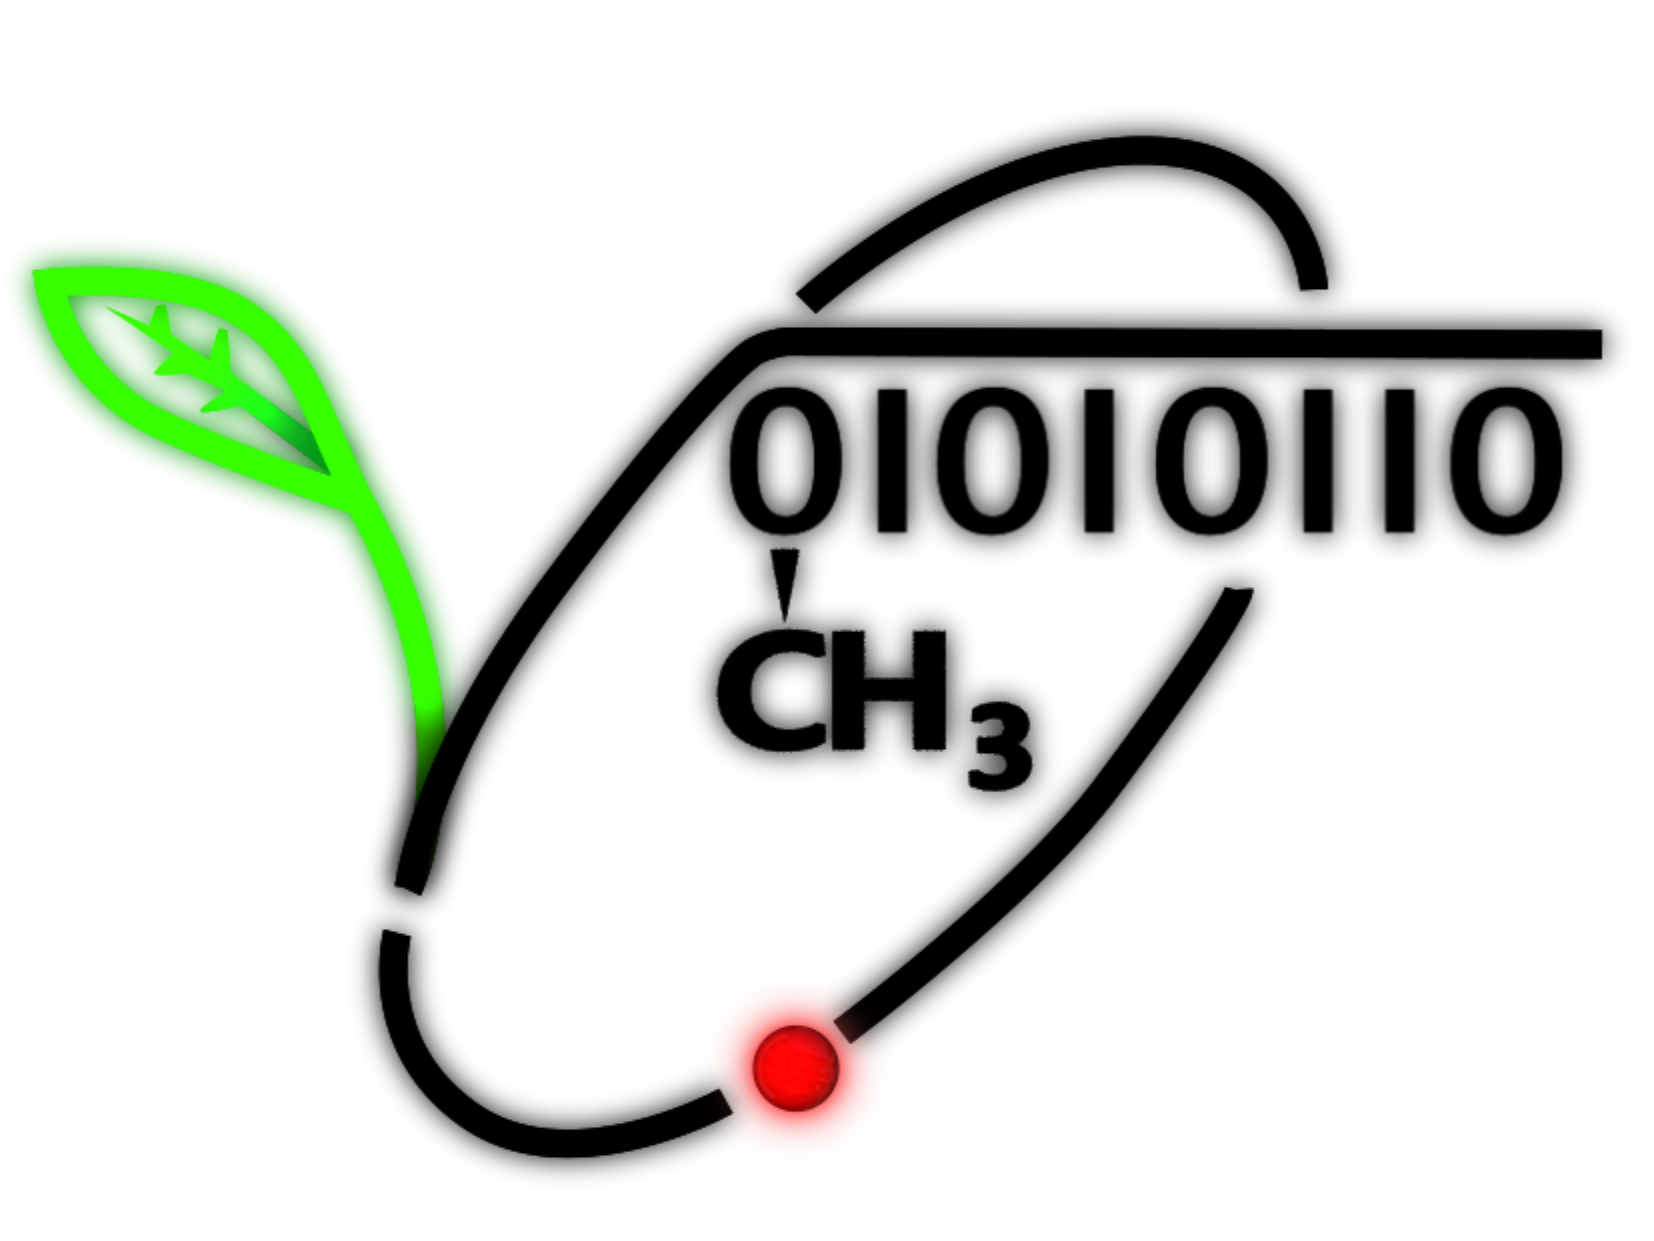
\includegraphics[width=0.5\textwidth]{pics/logo}\par\vspace{1cm}
	{\huge\bfseries Entwicklung eines Gamification-basierten Unterstützungs- und Motivationsgeräts zur Rehabilitation von Schlaganfall-Patienten\par}
	\vspace{2cm}
	{\large Seminarfacharbeit der \textsc{Klassenstufe 11/12} (Schuljahre 2017-2019)\\ am \\}
		{\scshape\Large\itshape Albert-Schweitzer-Gymnasium Erfurt, Spezialschulteil \par}
	\vspace{2cm}
	{\Large Lukas Rost}
	\vfill
	{\begin{tabular}{ll}
	\Large Fachbetreuer: & \Large Johannes Süpke \\[5pt]
	\Large Seminarfachbetreuer: & \Large Dr. Marion Moor \\[5pt]
	\Large Außenbetreuer: & \Large Hannes Weichel \\
	\end{tabular}}
	\vfill
	{\Large 20. Dezember 2018\par Erfurt}
\end{titlepage}

\newpage

%table of contents
\tableofcontents
\setcounter{page}{1}
\newpage

\section{Einleitung}
\glqq [Der Schlaganfall ist] nach Herzerkrankungen und Krebsleiden [...] die dritthäufigste Todesursache in Deutschland.\grqq\cite{Src:ApoFlex} So gab es im Jahr 2015 rund 40000 Todesfälle durch einen Schlaganfall oder seine Folgen.\cite{Src:Destatis} Doch viele der Betroffenen überleben glücklicherweise, tragen dabei jedoch Langzeitbehinderungen davon. So ist er sogar die häufigste Ursache für diese. \\ \\
Für die davon betroffenen Patienten bedeutet das langwierige Bewegungsübungen, bei denen der Erfolg noch nicht einmal sicher ist. In Studien wurde beispielsweise festgestellt, dass nur 5 Prozent der Patienten nach einer solchen Therapie wieder in der Lage waren, ihre Arme und Hände uneingeschränkt einzusetzen, während bei 20 Prozent der Patienten keine Hand- und Armfunktion zurückkehrte.\cite{Src:RehabNelles} \\ \\
Um eine solche Rehabilitation so erfolgreich wie möglich zu gestalten, existieren verschiedene Methoden, die in dieser Arbeit auch kurz vorgestellt werden sollen. Ihnen ist jedoch eines gemeinsam: Sie legen wenig Wert darauf, den Patienten zu unterstützen, zu motivieren und möglicherweise den Heilungsprozess durch solche positiven Wirkungen zu vereinfachen und zu beschleunigen. Dabei gibt es Methoden, die in dieser Hinsicht vielversprechend klingen, zum Beispiel die Gamification, auch Spielifizierung genannt. Bei dieser werden spieltypische Elemente in fremde Kontexte wie hier eine Therapie integriert, wodurch motivierende Wirkungen erzielt werden können. \\ \\
Ausgehend von dieser Überlegung soll in dieser Arbeit ein Gerät entwickelt werden, das bei der Therapie einer Armlähmung unterstützend wirken kann. Es soll Patienten motivieren, unterstützen und gegebenenfalls Hinweise bezüglich des Behandlungsfortschritts geben. Das Gerät benutzt dazu einen Elektromyografie-Sensor, der mittels Oberflächenelektroden die Kontraktion der Armmuskeln messen kann. Über Bluetooth-Funk werden diese Sensordaten an ein Smartphone übertragen, das der Patient mit einer zugehörigen Begleitapp benutzen kann. \\ \\
Diese App nutzt Methoden der Gamification wie Erfahrungspunkte oder Aufgaben (\glqq Quests\grqq), um die Motivation des Patienten bei solch monotonen Übungen zu steigern. Bezogen auf den Aufbau soll sie ähnlich wie eine konventionelle Fitness-App die Möglichkeit bieten, Übungen durchzuführen und auszuwerten. Nicht zuletzt soll sie es auch erlauben, ein Minispiel zu spielen, welches durch Armbewegungen gesteuert werden kann. \\ \\
Um die Motivation des Patienten über längere Zeit zu erhalten, sollen Benachrichtigungen den Nutzer, falls gewünscht, täglich an seine Übungen erinnern. Doch da die beste technische Lösung ohne die Einbindung in eine medizinisch anerkannte Therapie sinnlos ist, soll diese Arbeit auch auf Möglichkeiten dazu eingehen. \\ \\
Besonders danken möchte ich meinem Projektbetreuer Herrn Johannes Süpke, der mich im Prozess der Erstellung der Arbeit sowohl bei inhaltlichen und fachlichen Fragen als auch bei der Bereitstellung der nötigen Hardware unterstützte. Weiterhin gilt mein Dank meiner Seminarfachbetreuerin Frau Dr. Marion Moor für die Unterstützung in formalen, rhetorischen und sprachlichen Fragen. \\ \\
Außerdem möchte ich meinem Außenbetreuer Herrn Hannes Weichel danken, der mich mit wichtigen Vorschlägen zu Thema und Konzept der Arbeit sowie mit der Bereitstellung eines Mikrocontrollers und weiterer Materialien unterstützte. Nicht unerwähnt bleiben sollen jedoch auch Herr Frank Paulig und das SFZ Erfurt sowie Herr Udo Weitz und der Sponsorpool Thüringen des Wettbewerbs \glqq Jugend forscht\grqq , die die nötigen finanziellen Mittel für die Beschaffung noch nicht vorhandener Hardware bereitstellten.

\newpage
\section{Die Erkrankung Schlaganfall und geeignete Therapiemethoden}
\subsection{Schlaganfall als Krankheitsbild}
Beim Schlaganfall, auch \textit{Apoplexia cerebri} genannt, handelt es sich allgemein um eine \glqq plötzliche Durchblutungsstörung im Gehirn.\grqq ~\cite{Src:ApoNetdokt} Durch diese kommt es zu einem regionalen Mangel an Sauerstoff und Nährstoffen, welcher zu einem Absterben von Gehirngewebe führt.
\\ \\
Es existieren zwei mögliche Ursachen: Der ischämische oder Hirninfarkt tritt bei 80 bis 85 \% der Fälle auf. In diesem Fall ergibt sich eine mangelnde Durchblutung aufgrund von Gefäßverschlüssen, auch unter dem Begriff Arteriosklerose oder Thrombose zusammengefasst. Folgend kann es dabei zusätzlich auch zu einem Schlaganfall der zweiten Art kommen, dem sogenannten hämorrhagischen Infarkt bzw. der Hirnblutung, die 10 bis 15 \% der Fälle zugrundeliegt. Dieser wird durch geplatzte und eingerissene Gefäße verursacht, aus denen Blut ins Hirngewebe austritt. Dieses schädigt durch eine verminderte Sauerstoffversorgung, seinen Druck sowie seine neurotoxische Wirkung das Gehirn. Ein solcher Infarkt kann seinerseits wiederum eine Ischämie verursachen.\cite{Src:ApoFlex}
\\ \\
Im Vorfeld eines Schlaganfalls treten oft transitorisch-ischämische Attacken, also vorübergehende neurologische Ausfälle, auf. Symptome eines Schlaganfalls reichen von halbseitigen Körperlähm-ungen über Sprachstörungen und eingeschränktes Sprachverständnis (motorische und sensorische Aphasie) bis zu Sehstörungen und Gleichgewichtsproblemen. Auch Verwirrtheit, Übelkeit und Kopfschmerzen können auftreten.\cite{Src:ApoFlex}
\\ \\
Zur Erkennung von Schlaganfällen wird meist der FAST-Test benutzt, der fachsprachlich unter dem Begriff \glqq Cincinnati Prehospital Stroke Scale\grqq ~bekannt ist.\cite{Src:ApoWiki} Dieser besteht aus folgenden Punkten:
\begin{enumerate}
\item \textbf{F}ace/Gesicht: Person kann nur mit einer Gesichtshälfte lächeln
\item \textbf{A}rms/Arme: Unfähigkeit, beide Arme mit nach oben geöffneten Handflächen nach vorne zu strecken
\item \textbf{S}peech/Sprache: undeutliche Aussprache, kann nicht sprechen, versteht nichts mehr
\end{enumerate}
Sollten diese Punkte zutreffen, zählt der vierte Punkt: \textbf{T}ime (Zeit). Der Rettungsdienst sollte umgehend verständigt werden, um den Schaden zu begrenzen, denn \glqq Zeit ist Hirn \grqq.\cite{Src:ApoFlex}\footnote[2]{siehe \autoref{fig:fasttest}}
Die Diagnostik erfolgt in einer geeigneten Klinik mit \glqq Stroke Unit\grqq .~Dabei werden meist Verfahren wie Computertomografie und Magnetresonanztomografie genutzt. Die Schwere des Schlaganfalls wird mit Scoresystemen wie der \glqq National Institutes of Health Stroke Scale\grqq ~beurteilt.
\\ \\
Risikofaktoren umfassen unter anderem Bluthochdruck, Rauchen, Diabetes sowie Übergewicht und Bewegungsmangel. Dementsprechend wirkt eine gesunde Lebensweise präventiv. Dazu gehören gesunde Ernährung und regelmäßige Bewegung sowie ausreichende Flüssigkeitsaufnahme, aber auch Stressvermeidung.\cite{Src:ApoFlex} Es existieren jedoch auch andere, nicht beeinflussbare Risikofaktoren wie Alter, Blutgruppe und genetische Veranlagung.
\\ \\
Zu den Basismaßnahmen bei der Therapie gehört als erstes die Stabilisierung der Vitalfunktionen wie Blutdruck, Puls und Körpertemperatur. Auch sollte der Patient mit erhöhtem Oberkörper gelagert werden. Diese Maßnahmen stabilisieren den Patienten und dienen der Verhinderung eines weiteren Schlaganfalls. Weiterhin kann bei einem ischämischen Infarkt bis zu drei Stunden nach Auftreten des Schlaganfalls abhängig von der Größe des Infarkts eine intravenöse Thrombolyse-Therapie durchgeführt werden, um eventuell verschlossene Blutgefäße wieder zu öffnen. Bei Hirnblutungen dagegen sind operative Behandlungen sinnvoll, beispielsweise zur Hirndruck-Entlastung.\cite{Src:ApoFlex}
\subsection{Rehabilitation und Effektivität von Bewegungsübungen}
Armlähmungen zählen zu den häufigsten Folgen einer Hirnschädigung, wie sie durch einen Schlaganfall hervorgerufen wird.\cite{Src:DGNeurorehab} Aber auch Lähmungen anderer Körperteile oder Aphasie können auftreten.\cite{Src:ApoWiki} Meist betrifft eine solche Hirnschädigung nur eine Gehirnhälfte, sodass es nur auf einer Körperseite zu Lähmungen kommt. \\ \\
Die meisten Rehabilitationsmaßnahmen dienen dazu, die Körperwahrnehmung des Patienten zu fördern und verlorene Fähigkeiten zu kompensieren. Dabei sind Ansätze wie die \glqq Constraint-Induced Movement Therapy\grqq ~vielversprechend. Bei dieser auch als \glqq Taubsche Bewegungsinduktion\grqq ~bekannten Methode wird der gesunde Arm täglich über längere Zeit immobilisiert und der Betroffene somit gezwungen, die erkrankte Hand zu benutzen.\cite{Src:ApoWiki} So kann ein \glqq erlernter Nichtgebrauch\grqq ~verhindert werden. \cite{Src:RehabNelles}\\ \\
Ein weiteres bekanntes Rehabilitationskonzept ist das Bobath-Konzept, welches annimmt, dass gesunde Hirnregionen die Aufgaben geschädigter Hirnregionen übernehmen können. Durch das Konzept soll eine entsprechende Vernetzung innerhalb des Gehirns gefördert und die vom Schlaganfall betroffene Körperseite wieder in Bewegungen einbezogen werden.\cite{Src:BobathFlex} Solche Ansätze erfordern interdisziplinäre Zusammenarbeit. So können beispielsweise mit Physiotherapeuten Gangmuster eingeübt werden, während Ergotherapeuten an der Wiederherstellung der sensomotorischen Fähigkeiten arbeiten und Logopäden mit Sprachtherapie die Aphasie behandeln.\cite{Src:ApoWiki} \\ \\
Armlähmungen als solches zeigen sich unter anderem in einer stark beeinträchtigten willentli-
chen Bewegungsfähigkeit, aber auch durch \glqq  erhöhte Muskelanspannung (,Spastik') mit einer Fehlstellung des Armes in Ruhe\grqq ~sowie der Schwierigkeit, den Arm passiv zu bewegen. \cite{Src:DGNeurorehab} Zunächst sollten Armlähmungen medizinisch beurteilt werden, wozu spezielle Verfahren wie der Fugl-Meyer-Test existieren. Auf diese soll hier jedoch nicht genauer eingegangen werden. \\ \\
Es existieren verschiedene Therapiemethoden mit und ohne Technikeinsatz.
Das bilaterale Training beispielsweise besteht darin, dass mit beiden Armen gleichzeitig symmetrische Bewegungen ausgeführt werden, sodass in beiden Armen eine gleichmäßige Bewegungsfähigkeit hergestellt wird. Es wird in verschiedenen Studien neutral bis positiv beurteilt.\cite{Src:DGNeurorehab} \\ \\
Das schädigungsorientierte Training zielt darauf ab, spezifische Behinderungen bei alltäglichen Tätigkeiten zu beheben. Es existieren zwei Formen. Das Arm-Basis-Training beübt alle Bewegungsmöglichkeiten des Arms, also Schulter, Ellenbogen, Handgelenk und Finger. Es ist dabei auf Patienten mit schweren Lähmungen ausgelegt.\cite{Src:DGNeurorehab} Das Arm-Fähigkeits-Training dagegen schult verschiedene Formen von Geschicklichkeit und wird bei leichten Lähmungen angewendet.\cite{Src:DGNeurorehab}Beide Formen dieses Trainings zeigen einen positiven Effekt.\cite{Src:RehabNelles} Das aufgabenorientierte Training stellt eine weitere Trainingsform dar, bei der über Bewegungsaufgaben aus dem Alltag die funktionellen Fähigkeiten des Arms wiederhergestellt werden sollen. Es wird neutral beurteilt.\cite{Src:DGNeurorehab}\\ \\
Doch auch ein Technikeinsatz kann bei einer solchen Therapie erfolgen. So existiert beispielsweise die Armrobot-Methode, bei der ein Roboter nicht selbständig ausführbare Bewegungen mechanisch unterstützt. In Bezug auf die Effektivität wird diese positiv beurteilt.\cite{Src:DGNeurorehab} Auch die neuromuskuläre Elektrostimulation ist eine mögliche Therapie, bei der ein Gerät per Elektromyographie Bewegungsversuche des Muskels erkennt und diesen daraufhin elektrisch stimuliert, was zu einer großen Bewegung führt.\cite{Src:DGNeurorehab} Die Therapie wurde neutral beurteilt.\cite{Src:RehabNelles} \\ \\
Ausgehend von diesen Informationen erschien es sinnvoll, das Gerät als Unterstützung für Arm-Basis- und Arm-Fähigkeits-Training zu konzipieren. Im Zuge einer Erweiterung könnten auch Ansätze wie Armrobot und Elektrostimulation einbezogen werden.

\newpage
\section{Umgesetzte Konzepte}
\subsection{Gamification}
\subsubsection{Grundlegende Mechanismen der Gamification}
Es existieren verschiedene Definitionen für Gamification. Beispielhaft sei hier die Definition nach Breuer zitiert, die besagt, dass es sich bei Gamification um die \glqq Verwendung von spieltypischen Mechaniken außerhalb reiner Spiele, mit dem Ziel, das Verhalten von Menschen zu beeinflussen\grqq \cite{Src:GamifKochOtt} handelt. Entsprechend werden Spielkonzepte verwendet, um die Nutzungsmotivation zu steigern und die Nutzer dazu zu bewegen, mehr oder länger mit einem Produkt zu arbeiten als ohne Gamification. Diese Technik wird innerhalb eines Produktes dazu verwendet, dessen Nutzung zu proklamieren. \cite{Src:GamifKochOtt} \\ \\
Indem spieletypische Merkmale außerhalb spielerischer Zusammenhänge verwendet werden, nutzt man den menschlichen Spieltrieb aus. Es werden positive Anreize gesetzt, um Menschen zu einem bestimmten Verhalten anzuregen, während der Nutzer ebenfalls vorhandene negative Anreize wie eine Bestrafung vermeiden will. \cite{Src:PlanetWissen} Es kommt zu einer \glqq Actio-et-Reactio\grqq -Erfahrung.\cite{Src:GamifKochOtt} Diese Gestaltung und die entsprechende motivationsssteigernde Wirkung lassen sich mithilfe von psychologischen Theorien erklären, auf welche hier jedoch nicht genauer eingegangen werden soll. Gamification an sich ist an sich ein relativ neues Phänomen und wurde auch erst in letzter Zeit umgesetzt. So wurde der Begriff erst 1978 durch Richard Bartle, einen britischen Informatiker und Computerspiel-Pionier, geschaffen. \cite{Src:PlanetWissen} \\ \\
Dieser postulierte auch, dass die Wirkung von Anreizen sich bei verschiedenen Menschen unterscheide. Er entwarf deshalb ein Spielertypen-Koordinatensystem, in dem er Menschen in vier Kategorien verortete, wobei ein Mensch mehreren Kategorien zugleich angehören kann.\cite{Src:Bartle} Im Einzelnen beschrieb er folgende Typen, von denen in einem gelungenen Spiel oder bei einer gelungenen Gamification möglichst viele eine passende Motivation finden sollten:
\begin{itemize}
\item die Erfolgstypen/Achiever, welche im Spiel nach konkreten Maßstäben möglichst viel erreichen wollen.\cite{Src:Bartle} 10 Prozent aller Menschen werden hauptsächlich diesem Typ zugeordnet. \cite{Src:GamifDesign}
\item die Geselligen/Socializer, denen Kontakte und Interaktionen mit Mitspielern, wie sie auch in klassischen Gesellschaftsspielen vorkommen, besonders wichtig sind.\cite{Src:Bartle} 75 Prozent aller Menschen sind vor allem Socializer.\cite{Src:GamifDesign} 
\item die Forscher/Explorer, deren Ziel es ist, möglichst viel zu entdecken und erkunden.\cite{Src:Bartle} Dieser Typ ist bei ca. 10 Prozent aller Menschen am meisten ausgeprägt.\cite{Src:GamifDesign}
\item die Killer, welche Wettbewerb, Wettkampf und Konflikt lieben. Damit sie motiviert sind, müssen andere verlieren und ihnen Respekt erweisen.\cite{Src:Bartle} Dieser Typ macht 5 Prozent aller Menschen aus.\cite{Src:GamifDesign}
\end{itemize}
Um Gamification mit Erfolg anwenden zu können, ist es wichtig, die Kriterien und Mechanismen zu kennen, die ein erfolgreiches Spiel hervorbringen. Wie also kann Gamification angewendet werden, um langweilige, frustrierende, monotone oder unbeliebte Tätigkeiten, wie die dieser Arbeit zugrundeliegende Armlähmungs-Therapie, einfacher und motivierender zu gestalten? Zunächst sollten klare Ziele und Regeln aufgestellt werden, anhand derer der Nutzer weiß, welche Rückmeldung er auf eine bestimmte Aktion bekommt. Diese sogenannte Resultatstransparenz führt zu einer gesteigerten Handlungsmotivation.\cite{Src:GamifKochOtt} Außerdem sollten immer neue Herausforderungen gewährleistet sein.\cite{Src:WwieWissen}\\ \\
Eine motivierende Wirkung erzielt man auch, indem man den Spieler immer oder möglichst leicht gewinnen lässt. Der Spieler sollte beim Spielen in einen \glqq Flow\grqq ~ kommen, der durch eine starke Fokussierung auf das Spiel gekennzeichnet ist.\cite{Src:GamifDesign} Dafür darf ein Spiel weder zu einfach noch zu schwierig sein. Eine Belohnung des Spielers in einem festgelegten Intervall führt zu einer schnellen Abnahme der Motivation. Stattdessen sollte man auf die sogenannte operante Konditionierung setzen, indem man in einem variablen Intervall und in variabler Menge belohnt.\cite{Src:GamifDesign} \\ \\
Ein Spiel kann nach dem MDA-Modell durch drei Bestandteile charaktisiert werden: Mechanics (Spielkomponenten und -funktionen), Dynamics (Interaktion zwischen Spieler und Spiel) und Aesthetics (Emotionen, die beim Spieler erzeugt werden).\cite{Src:GamifDesign} Von diesen kann der Entwickler nur die Mechanics mithilfe spieltypischer Mechanismen beeinflussen. Zu diesen zählen unter anderem:
\begin{itemize}
\item ein Punktesystem gemeinsam mit einer einsehbaren Rangliste (Highscore) bei Mehrspieler-Spielens. Mit diesen können Aktionen des Spielers bewertet werden. Ein Highscore erlaubt einfache Vergleiche durch z.B. eine metrische Punkteskala.\cite{Src:GamifKochOtt} Highscores können auch suggestiv eingesetzt werden, indem sie den Spieler möglichst in der Mitte der Liste zeigen und somit gleichzeitig belohnen und motivieren.\cite{Src:GamifDesign}
\item ein sichtbarer Status durch Titel oder Badges. Diese repräsentieren nach außen, dass der Spieler ein bestimmtes Ziel erreicht hat und bieten somit Vergleichs- und Wettbewerbsmöglichkeiten.\cite{Src:GamifKochOtt} Motivierend sind sie außerdem, da Menschen gerne sammeln. Sie sollten jedoch nicht zu viel eingesetzt werden.\cite{Src:GamifDesign}
\item entdeckbare Aufgaben (Quests), die dem Spiel ein Ziel und Struktur geben und dafür sorgen, dass das  Spiel das Interesse des Spielers behält. Wenn Spieler zur Lösung einer Aufgabe mit Mitspielern zusammenarbeiten müssen, kann dies sozial sehr stark motivieren.\cite{Src:GamifDesign}
\item eine Fortschrittsanzeige, die eine dynamische Visualisierung des bisherigen Erfolgs und noch zu erledigender Aufgaben erlaubt.\cite{Src:GamifKochOtt}
\item gegebenenfalls ein Epic Meaning, also die Arbeit an etwas Erstrebenswerten und an sinnvollen Zielen.\cite{Src:GamifKochOtt}
\end{itemize}
\subsubsection{Beispiele für die motivationssteigernde Wirkung}
Gamification kann erstaunliche Effekte erzeugen. Exemplarisch deutlich wurde das bei einer Reihe von Experimenten der schwedischen Werbeagentur DDB unter dem Namen \glqq The Fun Theory\grqq . Bei einem dieser Experimente wurde eine U-Bahn-Treppe so umgebaut, dass sie wie eine Klaviertastatur bei Bedienung mit den Füßen Töne erzeugte. \footnote[4]{siehe \autoref{fig:pianostairs}} Im Ergebnis wurde diese Treppe sogar öfter als die danebenliegende Rolltreppe benutzt. \cite{Src:PlanetWissen} \\ \\
Auch ein Flaschencontainer, der bunt blinkte, wenn Flaschen in die richtige Öffnung geworfen wurden, und der \glqq tiefste Mülleimer der Welt\grqq , der beim Hineinwerfen von Müll einen Pfiff und einen Aufprall ertönen ließ, stellen erfolgreiche Beispiele dar. Im genannten Mülleimer beispielsweise erhöhte sich die Müllmenge drastisch. \cite{Src:PlanetWissen} Der Spieledesigner Kevin Richardson schlug für dieses Experiment eine Radarfallenlotterie vor, bei der alle, die die Geschwindigkeitsbegrenzung einhielten, an einem Gewinnspiel um die Strafzahlungen der Raser teilnahmen. Als dieser Vorschlag umgesetzt wurde, sank die Geschwindigkeit an der kontrollierten Stelle um 20 \% \cite{Src:GamifDesign} \\ \\
Im wissenschaftlichen Umfeld kann Gamification ebenfalls die Motivation steigern und so bessere Ergebnisse erzielen. So gelang es beispielsweise einigen Gamern, mithilfe eines Tetris-Nachbaus innerhalb von zehn Tagen die Proteinstruktur des AIDS-Virus zu entschlüsseln, was die Wissenschaftler hinter dem Projekt 15 Jahre gekostet hätte. \cite{Src:DLFMotiv} Unternehmen versuchen ebenfalls, durch Gamification geeignete Mitarbeiter zu finden. So entwarf der Bayer-Konzern eine Karriere-App im Stil von Quizshows und die Management-Simulation \glqq BIMS Online\grqq , die dort nun zur Rekrutierung geeigneter Fachkräfte dienen. \\ \\
Selbst eine Universität hat Gamification schon ausprobiert: An der Indiana University wurde zeitweise nach einem Experience-Point-System statt nach Noten bewertet. \cite{Src:XPNoten} Ein weiteres Beispiel für gelungene Gamification findet sich bei Frage-Antwort-Websites wie Quora, Stack Exchange oder Stack Overflow, bei welchen andere Nutzer entsprechende Punkte für gute Antworten auf bestimmte Fragen verleihen können. Außerdem kann ein Fragesteller die beste Antwort auf seine Frage markieren. All dies führt dazu, dass die Qualität der Antworten meist konstant hoch ist. \cite{Src:GamifDesign} \\ \\
Die bei solchen Experimenten gewonnenen Beobachtungen legen zumindest empirisch nahe, dass Gamification eine motivationssteigernde Wirkung besitzt. Unter Wissenschaftlern ist dieses Thema jedoch strittig. Einige Studien belegen diese These, andere widersprechen ihr. So wurde in einem Experiment der TU München versucht, das Berufsfeld der Kommissionierung, welches noch relativ wenig automatisiert ist, zu gamifizieren. Im Ergebnis arbeiteten die Kommissionierer schneller und zufriedener als ohne Gamification. \cite{Src:WwieWissen} \\ \\
Bei einer amerikanischen Studie, die sich auf den Erfolg von Fitnessmaßnahmen mit und ohne Wearable fokussierte, kam man jedoch zu gegenteiligen Ergebnissen. Obwohl Wearables ein klassisches Beispiel für Gamification darstellen, war keine signifikant höhere Gewichtsabnahme zu messen. Die mit Wearable ausgestatteten Probanden verloren im Vergleich zur Kontrollgruppe über den Zeitraum von 24 Monaten meist sogar weniger Gewicht. \cite{Src:WearableMotiv}
\subsection{Biofeedback}
In unserem Körper kommt es durch Regulationsvorgänge ständig zu Veränderungen von messbaren Zustandsgrößen bei biologischen Vorgängen und Körperfunktionen. Diese sind der unmittelbaren Sinneswahrnehmung, also dem Bewusstsein, nicht zugänglich. Sie können jedoch mit technischen und elektronischen Hilfsmitteln beobachtbar gemacht werden, was fachsprachlich unter dem Begriff Biofeedback bekannt ist. \cite{Src:BiofeedWiki} Oft wird dieses Verfahren zur Rehabilitation von erlahmten Muskeln, wie z.B. bei einer Armlähmung, eingesetzt. \\ \\
Da solche Körperfunktionen dem Bewusstsein normalerweise nicht zugänglich sind, können sie auch nicht beeinflusst werden. Durch Biofeedback wird genau das jedoch möglich. Durch die Visualisierung der Messwerte für den Patienten kommt es zu einer Rückkoppelung und dieser kann Kontrolle über die Körperfunktion ausüben. Weiterhin können über die operante Konditionierung ganze Reiz-Reaktions-Muster erlernt werden. Insgesamt wird eine Bewusstseinsschärfung für die eigenen inneren Zustände erreicht und die Einflussnahme auf das Nervensystem somit vereinfacht. \cite{Src:BiofeedWiki} \\ \\
Die Messwerte können nicht nur visualisiert werden, sondern werden bei manchen Anwendungen auch als Töne dargestellt. Die oft kleinen und tragbaren Messgeräte, die beim Biofeedback benutzt werden, messen meist nichtinvasiv. \cite{Src:BiofeedWiki} Ihre Messergebnisse werden dann in einem Analog-Digital-Wandler konvertiert, gemittelt und verstärkt. Anschließend werden sie per kabelloser Bluetooth-Übertragung auf ein zur Darstellung geeignetes Gerät übertragen. \\ \\
Grundsätzlich können per Biofeedback viele Größen gemessen werden, wie beispielsweise Atem, Blutdruck, Blutwerte, der Hautwiderstand oder Gehirnströme. Im hier beschriebenen Anwendungsfall ist jedoch die Messung von Muskelpotentialen per Elektromyografie am sinnvollsten, da mit dieser die Beweglichkeit des Arms am besten erfasst werden kann. In vielen Fällen erzielt Biofeedback positive Ergebnisse, sodass es in manchen Fällen sogar eine Alternative zu Medikamenten sein kann. \cite{Src:BiofeedWiki}

\newpage
\section{Schaltung und Implementierung des Mikrocontroller-Systems}
\subsection{Aufbau der Schaltung}
Das Mikrocontroller-System, welches für das Aufnehmen und Übertragen der Messdaten zuständig ist, besteht im Wesentlichen aus vier Bestandteilen, die miteinander verbunden sind:
\begin{enumerate}
\item Dem \textbf{Grove EMG-Sensor} \cite{Src:EMGdetect}~, der per Elektromyografie Messungen über die Stärke der Armmuskel-Kontraktionen erhebt. Dabei wird die elektrische Muskelaktivität anhand von Potentialänderungen auf der Haut mithilfe von drei Oberflächenelektroden gemessen. Diese Signale werden durch den Sensor verstärkt und gefiltert. Zuletzt gibt dieser eine Spannung im Bereich von 1,5 bis 3,3 Volt aus, wobei eine höhere Spannung höhere Muskelaktivität bedeutet. Dabei wird eine Versorgungsspannung von 3,3 bis 5 Volt benötigt.
\item Dem Mikrocontroller \textbf{Atmel ATmega 88PA} \cite{Src:AtmelDBeins}~, welcher die vom EMG-Sensor gelieferten Daten an den Bluetooth-Chip weitergibt. Es handelt sich hierbei um einen 8-Bit-Mikrocontroller\cite{Src:AtmelDBzwei}~, d.h. es können pro Takt maximal 8 Bit verarbeitet werden. Dieser folgt der sogenannten RISC-Architektur, welche einen reduzierten Befehlssatz im Vergleich zu Standardcomputern besitzt, dafür aber schneller arbeitet. Damit eignet er sich gut für den beabsichtigten Einsatzzweck, bei dem Daten möglichst schnell auf das Mobilgerät übertragen werden sollen. \\
Weiterhin setzt dieser Controllertyp die Harvard-Struktur um. \cite{Src:SchmittAVR} Es existieren also getrennte Speicher- und Adressbereiche für Befehle und Daten. Die peripheren Schnittstellen können über Portadressen angesprochen werden. Zu diesen Schnittstellen zählen zwei für die beabsichtigte Anwendung nötige, denn es werden sowohl eine UART-Schnittstelle zur Kommunikation mit dem Bluetooth-Chip als auch ein Analog-Digital-Wandler zum Einlesen der Ausgangsspannung des EMG-Sensors angeboten. Das Programm kann bei diesem Controller über ein Entwicklungsgerät in den Programmspeicher (Flash) geladen werden.
\item Dem Bluetooth-Chip \textbf{HC-05} \cite{Src:BluetoothHC}~, welcher eine Möglichkeit zur drahtlosen Kommunikation mit dem Android-Mobilgerät über Funk nach dem Bluetooth-Standard bereitstellt. Dabei sind alle zur Kommunikation nötigen Bestandteile auf einem Chip integriert. Der HC-05 wird über die UART-Schnittstelle (Universal Asynchronous Receiver Transmitter) angesprochen, wobei diese eine digitale serielle Schnittstelle zur Datenübertragung realisiert. Der Bluetooth-Chip kommuniziert standardmäßig mit 9600 Baud.
\item Einem \textbf{Quarzoszillatoren} mit eingebautem Schwingquarz, in diesem Fall mit der Frequenz 8 MHz, welcher einen genauen Systemtakt für den Mikrocontroller liefert. Dieser wird benötigt, um eine möglichst störungsfreie UART-Kommunikation realisieren zu können. Der Oszillator muss in den Einstellungen (Fuses) des Mikrocontrollers als Taktquelle ausgewählt (\texttt{CKSEL}-Bit) und die interne Teilung des Taktes durch 8 abgeschaltet (\texttt{CKDIV8}-Bit) werden.
\end{enumerate}
Diese Bestandteile wurden nach dem auf der folgenden Seite sichtbaren Schaltplan (\autoref{fig:mikrocontroller}) verbunden.
\subsection{Entwicklung des Programms auf dem Mikrocontroller}
Das Programm (siehe \autoref{listing:mikrocontroller}, S. \pageref{listing:mikrocontroller}) wurde in der Programmiersprache C geschrieben und besteht aus sechs Funktionen, die jedoch auf einige in den C-Standardbibliotheken vorhandene Funktionen und Definitionen für den C-Präprozessor zurückgreifen. Zusätzlich tätigt das Programm auch einige eigene Definitionen für den Präprozessor. Alle Funktionen außer der Main-Funktion, mit der das Programm startet, werden dem Compiler zunächst als Funktionsprototypen mithilfe ihrer Signaturen bekanntgemacht und erst nach der Main-Funktion definiert. Im einzelnen sind folgende Funktionen definiert:
\begin{itemize}
\item \texttt{init()}. Diese Funktion initialisiert die einzelnen Funktionen des Controllers, indem sie die entsprechenden Einstellungsregister \cite{Src:AtmelDBeins} setzt. Der Analog-Digital-Wandler wird aktiviert und dessen interner Taktteiler gesetzt. Die Sende- und die Empfangsfunktion der UART-Schnittstelle werden ebenfalls aktiviert und deren Baudratenfaktor, der angibt, wie schnell kommuniziert werden soll, gesetzt.
Der Baudratenfaktor \cite{Src:AtmelDBeins} berechnet sich aus (gerundet): \[UBBR = \frac{f_{CPU}}{16 \cdot r_{BAUD}} - 1 \]
Anschließend werden beide Schnittstellen zum ersten Mal ausgelesen, um ihre Funktionsfähigkeit sicherzustellen.
\item \texttt{u\_putch()}. Hier werden einzelne Zeichen (\textit{Char}) über die UART-Verbindung übertragen. Dabei muss gewartet werden, bis diese Verbindung freigegeben wird.
\item \texttt{u\_puts()}. Diese Funktion überträgt Zeichenketten (\textit{String}) über UART. Hierzu wird über die einzelnen Zeichen mithilfe der in C integrierten Zeigerarithmetik iteriert und jeweils \texttt{u\_putch()} aufgerufen.
\item \texttt{delay()} lässt den Mikrocontroller für die angegebene Zahl an Sekunden warten. Dazu wird die in der Bibliothek \texttt{util/delay.h} definierte Funktion \texttt{\_delay\_ms()} benutzt.
\item \texttt{sendCurrentVoltage()}. In dieser Funktion wird eine Analog-Digital-Wandlung gestartet und nach deren Abschluss das Ergebnis ausgelesen. Dabei handelt es sich um einen relativen Wert im Vergleich zur Referenzspannung \cite{Src:AVRTutor}, weshalb die eigentliche Spannung aus der Gleichung $U = \frac{x}{1024} \cdot U_{ref}$ gewonnen wird.\footnote{Hierbei ergibt sich jedoch insoweit ein Problem, als dass die Versorgungsspannung bei Batteriebetrieb schwanken kann.} Die dabei entstandene Gleitkommazahl wird mithilfe der Bibliotheksfunktion \texttt{sprintf()} in einen String geschrieben, der per \texttt{u\_puts()} übertragen werden kann.
\item \texttt{main()}. In dieser Funktion wird zuerst \texttt{init()} aufgerufen. Anschließend wird in einer Endlosschleife im Abstand einer halben Sekunde \texttt{sendCurrentVoltage()} gestartet und die Spannung an das Mobilgerät übertragen. Es muss sich hier um eine Endlosschleife handeln, da der Mikrocontroller nach der Ausführung von \texttt{main()} in ein undefiniertes Verhalten übergeht, aus dem er nur durch Neustart befreit werden kann.
\end{itemize}
\begin{figure}[H]
\centering
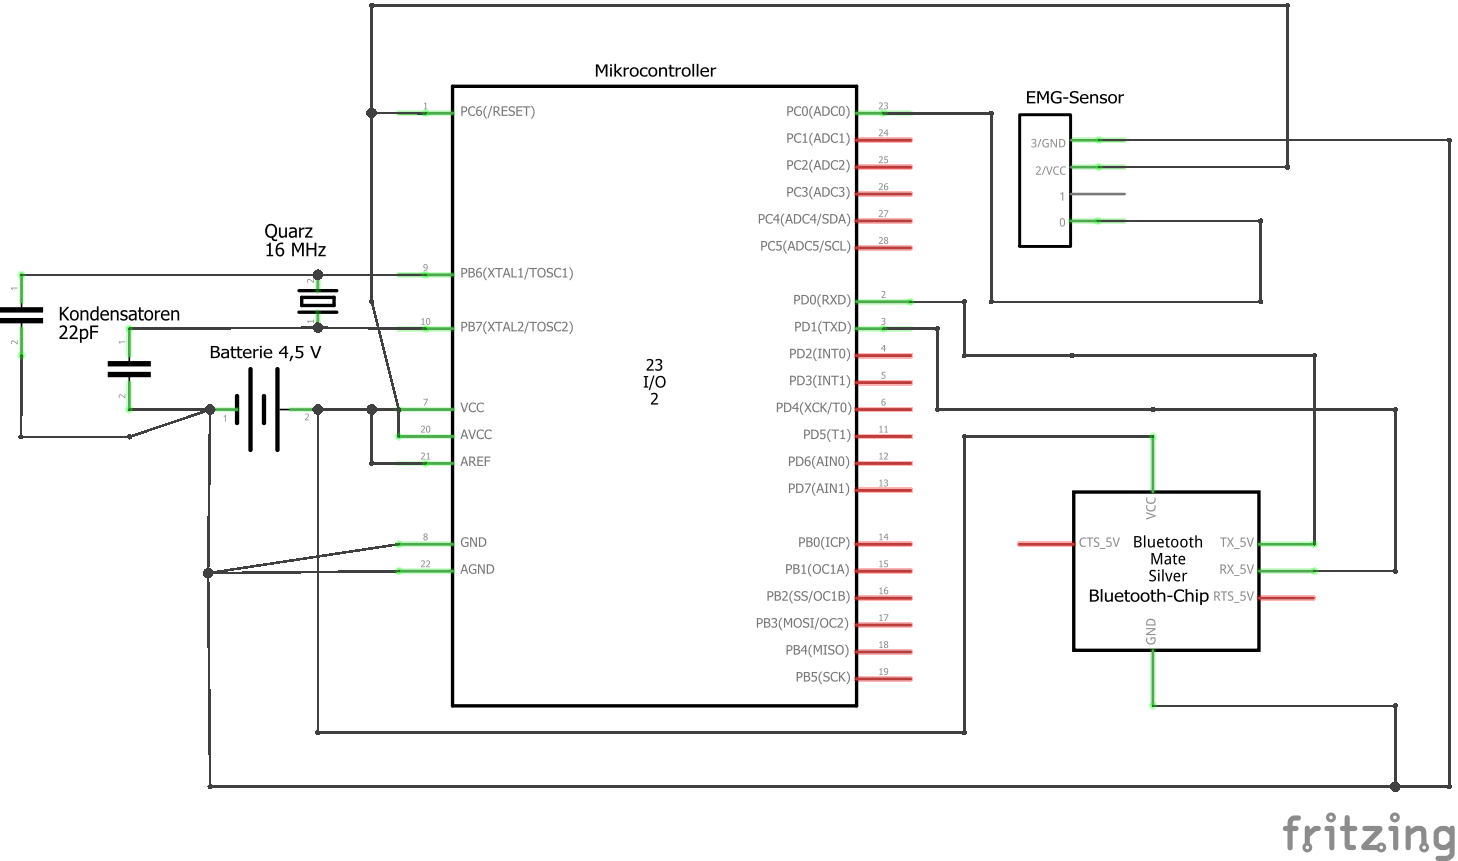
\includegraphics[width=0.8\textwidth]{pics/mikrocontroller_schaltplan.png}
\caption{Der Schaltplan des Mikrocontrollers. Einige Verbesserungen, um Rauschen aus dem Signal zu entfernen, sind der Einfachheit halber nicht dargestellt.}
\label{fig:mikrocontroller}
\end{figure}

\newpage
\section{Entwicklung der Begleitapp für Android}
\subsection{Grundlegender Aufbau und Konzept der App}
Um die vom EMG-Sensor gelieferten Daten zu verarbeiten und dem Benutzer bzw. Patienten anschaulich darzustellen, erschien es sinnvoll, eine App für Mobilgeräte zu programmieren. Hierbei fiel die Entscheidung, das weitverbreitete Betriebssystem Android zu verwenden und die App zu diesem (ab Android 6.0) kompatibel zu machen, wobei zur Umsetzung die Programmiersprache Kotlin\cite{Src:Kotlin} verwendet wurde. Diese App sollte folgende grundlegende Funktionen enthalten:
\begin{itemize}
	\item \textbf{Durchführung von Bewegungsübungen:} Es sollten einfache Bewegungsübungen möglich sein, bei denen sowohl der aktuelle Messwert als auch die Messwerte im zeitlichen Verlauf angezeigt werden sollten. Dabei sollte auch ein Vergleich mit früheren Übungen möglich sein.
	\item \textbf{Ein durch Bewegungsübungen steuerbares Minispiel:} Die App sollte ein durch den Benutzer mithilfe von Bewegungen steuerbares Minispiel enthalten. Dieses sollte möglichst einfach verständlich sein.
	\item \textbf{Ein verbindendes Gamification-System:} Sowohl bei normalen Übungen als auch beim Minispiel sollten Gamification-Elemente eingebracht werden. So sollte das Sammeln von Erfahrungspunkten (Experience Points, XP) möglich sein und es sollten für besondere Leistungen sogenannte Badges (Abzeichen) vergeben werden können. Dabei sollten die zu erbringenden Leistungen für die Badges in Form von Quests bzw. Aufgaben vorher für den Benutzer sichtbar sein.
	\item \textbf{Erinnerungen an die Übungen:} Die App sollte den Benutzer zu von ihm festgelegten Zeiten durch z.B. eine Benachrichtigung an die Durchführung seiner Übungen erinnern.
\end{itemize}
Ausgehend davon bot sich eine Gliederung in insgesamt vier für den Anwender sichtbare und miteinander verknüpfte Bildschirmseiten (bei Android Activities\cite{Src:AndroidKuenneth} genannt) an. Dies sind:
\begin{itemize}
	\item Eine \textbf{Startseite}, die die bisher erreichten Gamification-Erfolge zusammenfasst und kurze Informationstexte sowie Verknüpfungen zu den Übungsmöglichkeiten anbietet. Damit soll der Einstieg möglichst einfach gestaltet werden. Um die einzelnen Bereiche klar voneinander zu unterscheiden, kommt hier das einer Karteikarte ähnelnde Oberflächenelement \texttt{CardView} zum Einsatz.
	\item Eine \textbf{Übungsseite}, auf der man Übungen durchführen kann. Dabei zeigt ein tachoähnliches Oberflächenelement den aktuell festgestellten Messwert an, während mithilfe eines Diagramms die Messwerte während der gesamten Übung dargestellt werden. Diese Übung kann durch den Benutzer beliebig gestartet und beendet werden, während diese Seite auch eine Funktion zur Ansicht der aktuell verfügbaren Quests bereitstellt.
	\item Eine Seite für das \textbf{Minispiel}. Da dieses in einem späteren Abschnitt noch genauer beschrieben wird, soll hier nicht darauf eingegangen werden.
	\item Eine \textbf{Einstellungsseite}. Hier können Einstellungen getroffen werden, die für die restlichen Teile der App von Bedeutung sind. So kann man hier den eigenen Namen einstellen, die Gamification-Datenbank importieren und exportieren und die Übungserinnerungen konfigurieren. Für solche Seiten stellt das Android-SDK die Klasse \texttt{PreferenceFragment}\cite{Src:AndroidKuenneth} bereit.
\end{itemize}
Activities werden von Android intern auf dem sogenannten \textit{Back Stack} verwaltet, der basierend auf den abstrakten Datentyp Stack ein Zurückkehren zur vorherigen Activity erlaubt. Allgemein ist beim Arbeiten mit Activities das Lebenszyklus-Modell zu beachten, das beschreibt, auf welche Weise Activities gestartet, pausiert und gestoppt werden können.\cite{Src:AndroidKuenneth} Die einzelnen Bestandteile der App sollen im folgenden näher erläutert werden. Screenshots der jeweiligen Activities befinden sich im Anhang.
\newpage
\subsection{Kommunikation mit dem Mikrocontroller}
Wie bereits erläutert, sendet der Mikrocontroller die Messdaten über eine Bluetooth-Verbindung. Um nun mit  diesem kommunizieren zu können, muss die Android-App eine solche Verbindung implementieren. Glücklicherweise enthält das Android-SDK (Software Development Kit) bereits eine Softwarebibliothek, die genau dies vereinfacht.\cite{Src:AndroidBT} \cite{Src:AndroidKuenneth} \\ \\
Um eine Verbindung herzustellen, müssen zunächst einige Schritte durchlaufen werden, die nur in den Activities durchgeführt werden können. In dieser App benötigen zwei Activities Bluetooth-Zugriff: die Übungsseite und die Minispiel-Seite. Beide müssen unabhängig voneinander den Code zum Auffinden des zu verbindenden Bluetooth-Geräts implementieren. Dabei müssen beispielsweise die nötigen Berechtigungen überprüft, der Bluetooth-Adapter eingeschaltet und, sofern noch nicht geschehen, das Bluetooth-Gerät gekoppelt werden.\cite{Src:AndroidBT} \cite{Src:AndroidKuenneth} \\ \\
Ist dies geschehen, kann mit dem Einlesen der per Bluetooth über das Protokoll RFCOMM (Radio Frequency Communication)\cite{Src:AndroidKuenneth} eintreffenden Werte begonnen werden. Diese Funktionalität ist in der App in der Klasse \texttt{BluetoothNoService} gekapselt. Um kurzzeitige Schwankungen der Messwerte auszugleichen, bietet es sich an, diese in einer \textit{Queue} zwischenzulagern. Eine Queue oder Warteschlange ist eine in der Informatik häufig eingesetzte Datenstruktur, die nach dem First In - First Out - Prinzip (FIFO) arbeitet, d.h. das Objekt, welches als erstes der Warteschlange hinzugefügt wurde, verlässt sie auch als erstes wieder. Für diesen Zweck eignet sie sich sehr gut, da im Laufe der Zeit immer wieder neue Messwerte hinzukommen, während ältere entfernt werden müssen. Damit keine zu alten Werte verwendet werden, ist es sinnvoll, die Länge der Queue auf 4 Werte zu beschränken. \\ \\
Zum Hinzufügen der Werte ist es sinnvoll, einen Thread zu implementieren, d.h. eine Funktion, die parallel zum übrigen Programm abläuft. Dieser Thread kann der Queue dann beständig neue Werte hinzufügen, sobald diese eintreffen. \\ \\
Um nun zu jedem Zeitpunkt einen Durchschnittswert aus der Queue berechnen zu können, bietet sich der Mittelwert der Werte an. Da die Werte jedoch als Spannung abgelegt sind und der EMG-Sensor Werte zwischen $U_{min} = 1.5 V$ und $U_{max} = 3.3 V$ ausgibt, ist es sinnvoll, dem Nutzer die Werte in Prozent des Maximalwertes zu präsentieren. Ein solcher Wert lässt sich mit folgender Gleichung berechnen (wobei $x$ der Mittelwert der Messwerte ist):
\begin{equation*}
p = 100 * \frac{x - U_{min}}{U_{max} - U_{min}}
\end{equation*}
Dieser Wert kann nun an die Benutzeroberfläche zur weiteren Darstellung übergeben werden.
\subsection{Konzept und programmiertechnische Umsetzung des Minispiels}
Das Minispiel soll es erlauben, ein virtuelles Flugzeug über eine Gebirgslandschaft mit Bergen unterschiedlicher Höhe zu steuern. Dabei bestimmt die gemessene Muskelaktivität die Höhe des Flugzeugs. Je höher die Aktivität, desto höher fliegt das Flugzeug. Das Ziel ist es dabei, das Flugzeug möglichst lange fliegen zu lassen, ohne gegen einen Berg zu stoßen. Dieses Spielprinzip ähnelt teilweise dem erfolgreichen Smartphone-Spiel \glqq Flappy Bird\grqq . Es wäre wünschenswert, wenn es gelänge, an den Erfolg des genannten Spielprinzips anzuknüpfen. \\ \\
Zur Umsetzung des Minispiels wurde die Möglichkeit des Android-SDKs genutzt, eigene Oberflächenelemente (sogenannte \textit{Views}\cite{Src:CustomView}) zu erstellen. Eine solche View beinhaltet in diesem Fall das Spiel und übernimmt dessen Darstellung. Das Android-System fordert dabei, dass man bestimmte, für die eigene View spezifische Methoden überschreibt. Dies sind im einzelnen:
\begin{itemize}
	\item \texttt{onDraw()}: Hier wird der sichtbare Teil der View gezeichnet.\cite{Src:CustomView} \cite{Src:AndroidKuenneth} Was gezeichnet wird, hängt von der boolesche Objektvariable \texttt{inGame} der View ab, welche den Spielzustand (innerhalb oder außerhalb des Spiels) speichert. Befindet man sich außerhalb des Spiels, wird ein Text angezeigt, der darauf hinweist, dass durch einen Klick das Spiel gestartet werden kann. Innerhalb des Spiels müssen mehr Elemente gezeichnet werden. Zunächst jedoch wird der aktuelle Messwert des \texttt{BluetoothNoService} übernommen. \\ \\
	Nun werden anhand dieses Messwerts die Koordinaten der oberen linken Ecke des Flugzeugs bestimmt. Damit kann festgestellt werden, ob das Flugzeug gegen den Berg direkt vor ihm gestoßen ist. In diesem Fall ist das Spiel verloren. Ein entsprechender Infotext wird angezeigt und das Spiel durch die \texttt{handleTap()}-Methode beendet. \\ \\
	Ansonsten können der blaue Hintergrund, die grünen Berge sowie das als Icon vorliegende Flugzeug gezeichnet werden.
	\item \texttt{onSizeChanged()} und \texttt{onMeasure()}: Diese Methoden werden aufgerufen, wenn das System beispielsweise bei einer Drehung des Bildschirms eine Größenänderung der View anfordert.\cite{Src:CustomView} Entsprechend wird dann eine neue Höhe und Breite festgelegt. Daraufhin können alle von diesen abhängigen Teile der View neu generiert werden. Hier sind dies der Hintergrund und die zufällig (bezüglich ihrer Höhe) generierten Berge.
	\item \texttt{onTouchEvent()}: Diese Methode verarbeitet Touch-Eingaben bzw. Klicks. \cite{Src:InteractiveView} Android bietet dazu einen sogenannten \texttt{GestureDetector} an, der einfache und komplizierte Gesten erkennen kann. In diesem Fall muss jedoch nur das Tippen auf den Bildschirm erkannt und entsprechend das Spiel gestartet oder gestoppt werden. Dies übernimmt die Methode \texttt{handleTap()}.
\end{itemize}
\texttt{handleTap()} führt nun einige Schritte aus, die für das Starten bzw. Stoppen des Spiels nötig sind. Die bereits erwähnte \texttt{inGame}-Variable wird nun negiert, so dass der Spielzustand wechselt. Befindet man sich danach innerhalb des Spiels, so müssen nur die Höhen der Berge neu generiert werden. Dazu benutzt man einen einfachen Zufallsgenerator.\footnote[7]{Zunächst befinden sich jedoch über den Bereich einer Bildschirmbreite keine Berge, um den Spielstart zu vereinfachen.} \\ \\
Befindet man sich jedoch anschließend außerhalb des Spiels, so sind mehr Schritte durchzuführen. Die Liste der Berge sowie die Liste der Bluetooth-Messwerte müssen zurückgesetzt werden. Davor jedoch sollten entsprechende Gamification-Bewertungsfunktionen aufgerufen werden, die feststellen, wie viele XP beziehungsweise welche Badges der Nutzer für diese Leistung erhält. Die dazu nötigen Funktionen werden im nächsten Abschnitt genauer beschrieben. Nach den jeweiligen Änderungen wird die View natürlich neu gezeichnet. \\ \\
Das Android-Grafik-Framework unterscheidet beim Zeichnen im Übrigen dazwischen, was gezeichnet wird (bestimmt von der Klasse \texttt{Canvas}) und wie es gezeichnet wird (geregelt durch die Klasse \texttt{Paint}).\cite{Src:CustomView} Ein solches \texttt{Paint}-Objekt bestimmt dabei unter anderem Farbe, Stil und Schrift, die auf ein Objekt angewendet werden. Durch diese Teilung ist es möglich, \texttt{Paint}-Objekte schon vor der Benutzung zu erstellen und anschließend wiederzuverwenden. Da Views oft neu gezeichnet werden, kann dadurch die Performance verbessert und die Benutzeroberfläche flüssiger werden.\cite{Src:CustomView} \\ \\
Das fertige Spiel lässt sich nun folgendermaßen steuern: Zu Beginn erscheint der Text \glqq Um das Spiel zu beginnen, berühre den Bildschirm.\grqq Tippt man auf diesen, erscheint die Oberfläche des Spiels. Das Flugzeug kann auf dieser nun ausschließlich durch Muskelaktivität und nicht durch Touch-Gesten oder ähnliches gesteuert werden. Stößt man nun gegen einen Berg oder tippt man erneut auf den Bildschirm, wird das Spiel beendet, wobei im ersteren Fall ein zusätzlicher Hinweis (\glqq Du bist gegen einen Berg gestoßen. Du verlierst!\grqq) erscheint. Anschließend wird die für das Spiel zu vergebende XP-Punktzahl berechnet und angezeigt sowie auf eventuell abgeschlossene Quests überprüft.
\subsection{Umsetzung der Gamification in der App}
Im Bereich der Gamification fiel die Entscheidung, ein (Erfahrungs-)Punktesystem und Quests bzw. Badges einzuführen. Für jede durchgeführte Übung bzw. für jedes Spielen des Minispiels werden hier abhängig von den aufgenommenen Messwerten Punkte verteilt. Dabei gelten für die Verteilung folgende Kriterien:
\begin{itemize}
	\item Bei einer \textbf{Übung} wird eine Liste $L$ der prozentualen Messwerte erstellt. Aus dieser kann dann die Punktzahl $P$ berechnet werden:
	\begin{align*}
	P = \frac{min(L) + avg(L) + max(L)}{3}
	\end{align*}
	Dabei berechnet $min(L)$ den Minimalwert der Liste, $avg(L)$ den Durchschnittswert der Liste und $max(L)$ den Maximalwert der Liste.
	\item Beim \textbf{Minispiel} gelten die Regeln für eine Übung grundsätzlich weiter. Jedoch werden als Bonus zusätzlich $2 \cdot d$ XP vergeben, wobei $d$ die Anzahl der aufgenommenen Messwerte bis zum Absturz des Flugzeugs darstellt.
\end{itemize}
Natürlich wird der Nutzer auch jeweils über die vergebene Punktzahl mithilfe einer im unteren Bildschirmteil eingeblendeten \texttt{Toast}-Benachrichtigung informiert. \\ \\
Bei den bereits erwähnten Quests erschien es sinnvoll, verschiedene Kriterien bzw. Anforderungen für die Fertigstellung der Quest vorauszusetzen. Um diese bei den einzelnen Quests flexibel regulieren zu können, kann man solche Daten in einer lokalen Datenbank speichern, auf welche die App dann zugreifen kann. Android bietet dafür die sehr kompakte Datenbankbibliothek \textit{SQLite} an, welche ein relationales Datenbanksystem implementiert und über die standardisierte Datenbanksprache \textit{SQL} angesprochen werden kann.\cite{Src:AndroidKuenneth} Besonders wichtig ist hierbei, dass keine Server-Software benötigt wird, sondern die Datenbank einfach in einer einzelnen Textdatei gespeichert werden kann, was im Kontext einer Android-App vieles vereinfacht.\cite{Src:AndroidKuenneth} \\ \\
Die Datenbanktabelle besteht nun aus den folgenden Spalten, welche eine einzelne Quest kennzeichnen:
 \begin{longtabu} to \linewidth {|l|l|X|}
	\hline
	\textbf{Spaltenname} & \textbf{Spaltentyp} & \textbf{Beschreibung} \\[0.3em] \hline \endhead
	\texttt{\_id} & \texttt{INT} & Die eindeutige Identifikationsnummer der Quest, über die sie aufgerufen und verändert werden kann. \\[0.5em] \hline	
	\texttt{title} & \texttt{VARCHAR(50)} & Der Titel der Quest. Dieser kann bis zu 50 Zeichen lang sein. \\[0.5em] \hline
	\texttt{description} & \texttt{VARCHAR(150)} & Eine Beschreibung der Quest, die bis zu 150 Zeichen lang sein kann. Sie sollte möglichst die in den restlichen Spalten definierten Ziele zum Erfüllen der Quest zusammenfassen.  \\[0.5em] \hline
	\texttt{icon} & \texttt{INT} & Ein Zahl zwischen 1 und 5, die für die Anzeige der Quest eines von 5 vordefinierten Symbolen auswählt. \\[0.5em] \hline
	\texttt{requiredXP} & \texttt{INT} & Gibt den XP-Stand an, der zur Anzeige der Quest nötig ist. \\[0.5em] \hline
	\texttt{finishedXP} & \texttt{INT} & Gibt den XP-Stand an, der zum Beenden der Quest notwendig ist. \\[0.5em] \hline
	\texttt{earnedXP} & \texttt{INT} & Gibt die Anzahl an XP an, die der Nutzer für die Beendigung der Quest erhält. \\[0.5em] \hline
	\texttt{overPercentage} & \texttt{INT} & Gibt einen Messwert an, über dem man für eine bestimmte Zeit sein muss, um die Quest zu beenden. \\[0.5em] \hline
	\texttt{timeOverPercentage} & \texttt{INT} & Gibt die Zeitspanne an, während der man über dem genannten Messwert sein muss. \\[0.5em] \hline
	\texttt{minimumPercentage} & \texttt{INT} & Gibt eine Prozentzahl bzw. einen Messwert an, der mindestens einmal während einer Übung erreicht werden muss, um die Quest zu beenden. \\[0.5em] \hline
	\texttt{isCompleted} & \texttt{BOOL} & Gibt an, ob die Quest bereits beendet und damit in ein Badge umgewandelt wurde. \\[0.5em] \hline
\end{longtabu}
In allen INT-Spalten außer \texttt{\_id} und \texttt{icon} kann auch eine $0$ stehen. Dies bedeutet dann, dass die entsprechende Anforderung bei dieser Quest nicht benötigt wird. \\ \\
Nun ist es relativ einfach, die Quests und Badges in der App anzuwenden. Nach jeder Übung und jedem Spiel kann nun anhand der in der Tabelle festgelegten Kriterien überprüft werden, ob eine der Quests beendet wurde. Dazu müssen drei Bedingungen erfüllt sein: die \texttt{minimumPercentage}-Bedingung (der Wert wurde mindestens einmal erreicht), die \texttt{overPercentage}-Bedingung (der Wert wurde für die angegebene Zeitspanne überschritten) und ein entsprechender XP-Stand. \\ \\
Ist dies der Fall, kann die Quest durch eine Datenbankabfrage auf \glqq erledigt\grqq ~gesetzt werden. Die durch die Quest verdienten XP-Punkte können dem Nutzer nun gutgeschrieben werden. Gleichzeitig wird mithilfe eines \texttt{DialogFragment}s dem Benutzer ein Dialog angezeigt, der ihn über die abgeschlossenen Quests und die dafür erhaltenen Erfahrungspunkte informiert. \\ \\
Natürlich ist es dem Nutzer auch möglich, sich die erhaltenen Badges bzw. die zur Verfügung stehenden Quests anzuzeigen. Im ersteren Fall wird diese Funktion durch einen Button auf der Startseite aufgerufen, im letzteren Fall durch einen Button auf der Übungsseite. In beiden Fällen wird ein \texttt{Dialog} mit einer \texttt{ListView} angezeigt, die Elemente auflisten kann. Hier sind dies die Quests bzw. Badges, welche über einen \texttt{CursorAdapter} einfach aus der Datenbank abgerufen werden können. \\ \\
In Hinsicht auf die Umsetzung der Gamification ist jedoch auch zu betrachten, inwieweit die App der Gamification-Theorie folgt, um daraus möglicherweise Rückschlüsse auf die Wirksamkeit zu ziehen. Bezüglich der Spielertypen ist die App beispielsweise eher für Forscher und Erfolgstypen ausgelegt, da sich die Gamification-Elemente aktuell darauf fokussieren, den Nutzer Erfolge erreichen zu lassen. Nutzer dagegen, die im Bartle-Test eher als Gesellige oder Killer eingeordnet werden, haben wenig Möglichkeiten, mit anderen zu interagieren und mit ihnen in Wettbewerb zu treten, da eine Mehrspielerfunktion fehlt, welche den zeitlichen Rahmen der Arbeit gesprengt hätte. Die Einbindung einer solchen Funktion wäre jedoch eine Erweiterungsmöglichkeit. \\ \\
Jedoch ist die für Gamification wichtige Handlungstransparenz gegeben, da der Nutzer sich seinen XP-Stand und die verfügbaren Quests einfach ansehen kann. Neue Herausforderungen sind trotzdem nur begrenzt gegeben, da das Hinzufügen von Quests in der aktuellen Version noch schwierig ist. Dies ließe sich durch eine Updatefunktion über das Internet beheben. Das Minispiel ist weder zu einfach noch zu schwer, da es sich am bekannten Prinzip des Spiels \textit{Flappy Bird} orientiert. Das ermöglicht es dem Nutzer, in einen Flow zu kommen. \\ \\
Auch das Prinzip der operanten Konditionierung wurde umgesetzt, denn die Vergabe von Erfahrungspunkten und Badges erfolgt abhängig von den Messwerten immer unterschiedlich. Die Belohnung in einem variablen Intervall ist dabei jedoch nicht möglich, da die Vergabe nur jeweils nach einer Übung oder einem Spiel erfolgen kann. \\ \\
Im Bereich der spieltypischen Mechanismen wurden einige umgesetzt. So enthält die App, wie bereits beschrieben, ein Erfahrungspunkte-System. Ein Highscore jedoch ist aufgrund der fehlenden Mehrspieler-Möglichkeiten nicht vorhanden. Hingegen ist ein System aus Quests und Badges vorhanden, die so verknüpft sind, dass aus einer abgeschlossenen Quest ein Badge erzeugt wird. Damit existiert ein sichtbarer Status, der der App ein Ziel und eine Struktur gibt und den Fortschritt des Nutzers symbolisiert. Ein sinnvolles Ziel bzw. Epic Meaning ist hier in jedem Fall vorhanden, denn der Benutzer möchte seine Armlähmung bekämpfen.
\subsection{Funktionsweise des Benachrichtigungssystems}
Das Benachrichtigungssystem besteht aus einer Reihe von Funktionen, die vorrangig durch die Einstellungsseite gesteuert werden. Die erste dieser Funktionen erledigt eine seit Android 8 für das Senden von Benachrichtigungen nötige Maßnahme, indem sie einen Benachrichtigungskanal einrichtet. Mithilfe dessen ist es dem Benutzer möglich, die Benachrichtigungen über die Systemeinstellungen zu unterdrücken.\cite{Src:AndroidNotify} Tut er dies nicht, können die Benachrichtigungen über die Einstellungsseite der App reguliert werden.\\ \\
Eine weitere Funktion ist für das Setzen einer Erinnerung zuständig. Sie liest aus den Einstellungen (sogenannte \texttt{SharedPreferences}) aus, ob und wann erinnert werden soll. Nachdem alle bisherigen Erinnerungen gelöscht wurden, kann eine neue gesetzt werden. Dazu verwendet die App den System-Service \texttt{AlarmManager}\cite{Src:NotifyDroid}. Sobald die gewünschte Zeit erreicht wurde, ruft dieser einen \texttt{BroadcastReceiver} auf. Solche \texttt{BroadcastReceiver} sind ein fester Bestandteil des Android-SDK und können auf vielfältige Meldungen durch das Android-System, welche auf Systemereignisse hinweisen, reagieren.\cite{Src:AndroidKuenneth} In diesem Fall wird hier eine Methode zum Senden der Benachrichtigung aufgerufen. \\ \\
Wird eine solche Benachrichtigung gesendet, ist sie systemweit für den Nutzer sichtbar und erinnert ihn daran, seine Übungen durchzuführen. Bei Klick auf die Benachrichtigung öffnet sich die Startseite der App. \\ \\
Schließlich lassen sich, wie bereits erwähnt, sämtliche im \texttt{AlarmManager} gespeicherten Erinnerungen auch wieder löschen, wovon entsprechend der Einstellungen Gebrauch gemacht wird.\footnote[3]{Die Implementierung des Benachrichtigungssystems in \texttt{NotificationScheduler.kt} basiert teilweise auf einer in  \cite{Src:NotifyDroid} vorgestellten Lösung.}

\newpage
\section{Zusammenfassung}
Ausblick: "Die Rehabilitation [ist] ein großes Thema, also das Bewegungstraining bei Schlaganfallpatienten [...]." (Sami Haddadin in Interview zu Robotern) (Src:CTHaddadin)

\newpage
\renewcommand{\refname}{Literatur- und Quellenverzeichnis}

\begin{thebibliography}{xxxxxx}

\subsection*{Literaturquellen}

\bibitem[1] {Src:GamifDesign} Cunningham, Christopher; Zichermann, Gabe: \textit{Gamification by Design} - Implementing Game Mechanics in Web and Mobile Apps, 1. Auflage, Sebastopol, O'Reilly Verlag, 2011, online verfügbar unter \url{https://doc.lagout.org/programmation/Game Design/Gamification by Design - Zichermann, Cunningham - O'Reilly (2011)/Gamification by Design - Zichermann, Cunningham - O'Reilly (2011).pdf}

[Zugriff am 30.1.2018, 18:20 Uhr]

\bibitem[2] {Src:AndroidGargenta} Gargenta, Marko: \textit{Einführung in die Android-Entwicklung}, 1. Auflage, Köln, O'Reilly Verlag, 2011

\bibitem[3] {Src:CTHaddadin} Grävemeyer, Arne: \textit{Ära starker Bots mit zarten Fingern}, Roboterforscher Haddadin erwartet Wandel in Industrie und Haushalt, in: c't 11/2018, S. 68 - 69

\bibitem[4] {Src:Kotlin} Isakova, Svetlana; Jemerov, Dmitry: \textit{Kotlin in Action}, 1. Auflage, Shelter Island, Manning Publications, 2017

\bibitem[5] {Src:WearableMotiv} Jakicic, John M. et al.: \textit{Effect of Wearable Technology Combined With a Lifestyle Intervention on Long-term Weight Loss}, The IDEA Randomized Clinical Trial, In: Journal of the American Medical Association, 316(11)/2016, S. 1161 - 1171, online verfügbar unter \url{https://jamanetwork.com/journals/jama/articlepdf/2553448/joi160104.pdf}

[Zugriff am 27.12.2017, 15:37 Uhr]

\bibitem[6] {Src:AndroidKuenneth} Künneth, Thomas: \textit{Android 8 - Das Praxisbuch für Java-Entwickler}, 5. aktualisierte Auflage, Bonn, Rheinwerk Verlag, 2018

\bibitem[7] {Src:DGNeurorehab} Platz, Thomas; Roschka, Sybille: \textit{Rehabilitative Therapie bei Armlähmungen nach einem Schlaganfall}, Patientenversion der Leitlinie der Deutschen Gesellschaft für Neurorehabilitation, Bad Honnef, Hippocampus Verlag, 2011, 
online verfügbar unter \url{http://www.kompetenznetz-schlaganfall.de/fileadmin/download/Arm-Reha/Leitlinie_Therapie_Armlaehmung_220911-verlinkt.pdf} 

[Zugriff am 27.12.2017, 16:04 Uhr]

\bibitem[8] {Src:SchmittAVR} Schmitt, Günter: \textit{Mikrocomputertechnik mit Controllern der Atmel AVR-RISC-Familie}, Programmierung in Assembler und C - Schaltungen und Anwendungen, 4. Auflage, München, Oldenbourg Verlag, 2008

\subsection*{Internetquellen}

\bibitem[9]{Src:AndroidBT} Android Developer Team: \textit{Bluetooth overview}, \url{https://developer.android.com/guide/topics/connectivity/bluetooth}

[Zugriff am 11.11.2018, 15:36 Uhr]

\bibitem[10]{Src:AndroidNotify} Android Developer Team: \textit{Create a Notification}, \url{https://developer.android.com/training/notify-user/build-notification}

[Zugriff am 11.11.2018, 15:38 Uhr]

\bibitem[11]{Src:CustomView} Android Developer Team: \textit{Custom Drawing}, \url{https://developer.android.com/training/custom-views/custom-drawing}

[Zugriff am 11.11.2018, 15:40 Uhr]

\bibitem[12]{Src:InteractiveView} Android Developer Team: \textit{Making the View Interactive
}, \url{https://developer.android.com/training/custom-views/making-interactive}

[Zugriff am 11.11.2018, 15:43 Uhr]

\bibitem[13] {Src:ApoFlex} Antwerpes, Frank et al.: \textit{Schlaganfall}, \url{http://flexikon.doccheck.com/de/Schlaganfall}

[Zugriff am 31.12.2017, 12:35 Uhr]

\bibitem[14] {Src:AtmelDBeins} Atmel Corporation: \textit{ATmega48A/PA/88A/PA/168A/PA/328/P}, Atmel 8-Bit Microcontroller with 4/8/16/32 KBytes In-System Programmable Flash, Datasheet, \url{http://www.atmel.com/images/Atmel-8271-8-bit-AVR-Microcontroller-ATmega48A-48PA-88A-88PA-168A-168PA-328-328P_datasheet_Complete.pdf} 

[Zugriff am 27.12.2017, 11:46 Uhr]

\bibitem[15] {Src:AtmelDBzwei} Atmel Corporation: \textit{ATmega48PA/88PA/168PA}, 8-bit AVR Microcontrollers, Datasheet Complete, \url{http://ww1.microchip.com/downloads/en/DeviceDoc/Atmel-42734-8-bit-AVR-Microcontroller-ATmega48PA-88PA-168PA_Datasheet.pdf} 

[Zugriff am 27.12.2017, 11:48 Uhr]

\bibitem[16] {Src:AVRTutor} Autorengemeinschaft: \textit{AVR-GCC-Tutorial}, \url{https://www.mikrocontroller.net/articles/AVR-GCC-Tutorial}

[Zugriff am 27.12.2017, 12:10 Uhr]

\bibitem[17] {Src:Bartle} Autorengemeinschaft: \textit{Bartle-Test}, \url{https://de.wikipedia.org/wiki/Bartle-Test}

[Zugriff am 4.4.2018, 14:11 Uhr]

\bibitem[18] {Src:BiofeedWiki} Autorengemeinschaft: \textit{Biofeedback}, \url{https://de.wikipedia.org/wiki/Biofeedback}

[Zugriff am 5.4.2018, 16:25 Uhr]

\bibitem[19] {Src:ApoWiki} Autorengemeinschaft: \textit{Schlaganfall}, \url{https://de.wikipedia.org/wiki/Schlaganfall}

[Zugriff am 31.12.2017, 13:01 Uhr]

\bibitem[20] {Src:PlanetWissen} Drescher, Frank: \textit{Spiele und Spielzeug - Gamification}, \url{https://www.planet-wissen.de/gesellschaft/spiele_und_spielzeug/gamification/index.html}

[Zugriff am 30.3.2018, 10:12 Uhr]

\bibitem[21] {Src:ApoNetdokt} Feichter, Martina: \textit{Schlaganfall}, \url{https://www.netdoktor.de/krankheiten/schlaganfall/}

[Zugriff am 31.12.2017, 13:25 Uhr]

\bibitem[22]{Src:NotifyDroid} Fernando, Jaison: \textit{How to schedule notifications using AlarmManager?}, \url{https://droidmentor.com/schedule-notifications-using-alarmmanager/}

[Zugriff am 11.11.2018, 15:49 Uhr]

\bibitem[23] {Src:BobathFlex} Freyer, Timo; Mörkl, Sabrina; Ostendorf, Norbert: \textit{Bobath-Konzept}, \url{http://flexikon.doccheck.com/de/Bobath-Konzept}

[Zugriff am 3.1.2018, 17:42 Uhr]

\bibitem[24] {Src:BluetoothHC} ITead Studio: \textit{HC-05}, Bluetooth to Serial Port Module, \url{http://www.electronicaestudio.com/docs/istd016A.pdf}

[Zugriff am 27.12.2017, 11:13 Uhr]

\bibitem[25] {Src:GamifKochOtt} Koch, Michael; Ott, Florian: \textit{Gamification} – Steigerung der Nutzungsmotivation durch Spielkonzepte, Projekt mit der Forschungsgruppe Kooperationssysteme an der Universität der Bundeswehr München, \url{http://www.soziotech.org/gamification-steigerung-der-nutzungsmotivation-durch-spielkonzepte/}

[Zugriff am 30.1.2018, 18:03 Uhr]

\bibitem[26] {Src:XPNoten} Parrish, Kevin: Professor Uses RPG-like Exp Rather Than Grades, \url{https://www.tomsguide.com/us/Experience-Points-XP-Indiana-University,news-6183.html}

[Zugriff am 5.4.2018, 15:32 Uhr]

\bibitem[27] {Src:RehabNelles} Nelles, Gereon et al.: \textit{Motorische Rehabilitation nach Schlaganfall}, \url{http://www.friedehorst.de/nrz/rehabilitation.pdf?m=1140520827}

[Zugriff am 27.12.2017, 16:16 Uhr]

\bibitem[28] {Src:DLFMotiv} Reinhardt, Anja: \textit{Motivation und Manipulation im Alltag}, Spieltheorie \glqq Gamification\grqq , \url{http://www.deutschlandfunk.de/spieltheorie-gamification-motivation-und-manipulation-im.724.de.html}

[Zugriff am 5.4.2018, 15:59]

\bibitem[29] {Src:EMGdetect} Seeed Technology Co. Ltd.: \textit{Grove - EMG Detector}, \url{http://wiki.seeed.cc/Grove-EMG_Detector/}

[Zugriff am 30.12.2017, 14:03 Uhr]

\bibitem[30] {Src:Destatis} Statistisches Bundesamt: \textit{Ergebnisse der Todesursachenstatistik für Deutschland 2015}, ausführliche 4-stellige ICD10-Klassifikation, \\ \url{https://www.destatis.de/DE/Publikationen/Thematisch/Gesundheit/Todesursachen/Todesursachenstatistik5232101157015.xlsx?__blob=publicationFile}

[Zugriff am 2.1.2018, 11:16 Uhr]

\bibitem[31] {Src:WwieWissen} W wie Wissen: \textit{Gamification - Wie Spielen den Alltag interessanter macht}, Ausschnitt aus der gleichnamigen Sendung in Das Erste am 19.12.2015 (16.00 Uhr), \url{http://www.ardmediathek.de/tv/W-wie-Wissen/Gamification-Wie-Spielen-den-Alltag-in/Das-Erste/Video?bcastId=427262&documentId=32368232}

[Zugriff am 4.4.2018, 14:32 Uhr]
\end{thebibliography}


\newpage
\section{Anhang}
\renewcommand{\thesubsection}{\arabic{subsection}}
\setcounter{subsection}{2}
%\setcounter{figure}{0}
\tocless\subsubsection{Schlaganfall als Krankheitsbild}
\begin{figure}[H]
\centering
\includesvg[width=0.8\textwidth]{pics/Schlaganfall}
\caption{Schaubild zum FAST-Test}
\label{fig:fasttest}
\end{figure}

\setcounter{subsection}{3}
\setcounter{subsubsection}{0}
\tocless\subsubsection{Gamification}
\begin{figure}[H]
\centering
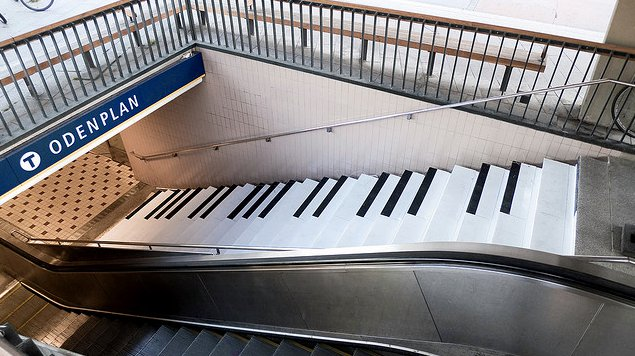
\includegraphics[width=0.8\textwidth]{pics/pianostairs.jpg}
\caption{Die Klavier-Treppe aus dem Projekt \emph{The Fun Theory}}
\label{fig:pianostairs}
\end{figure}


\setcounter{subsection}{4}
\setcounter{subsubsection}{0}
\tocless\subsubsection{Aufbau der Schaltung}
\begin{figure}[H]
	\centering
	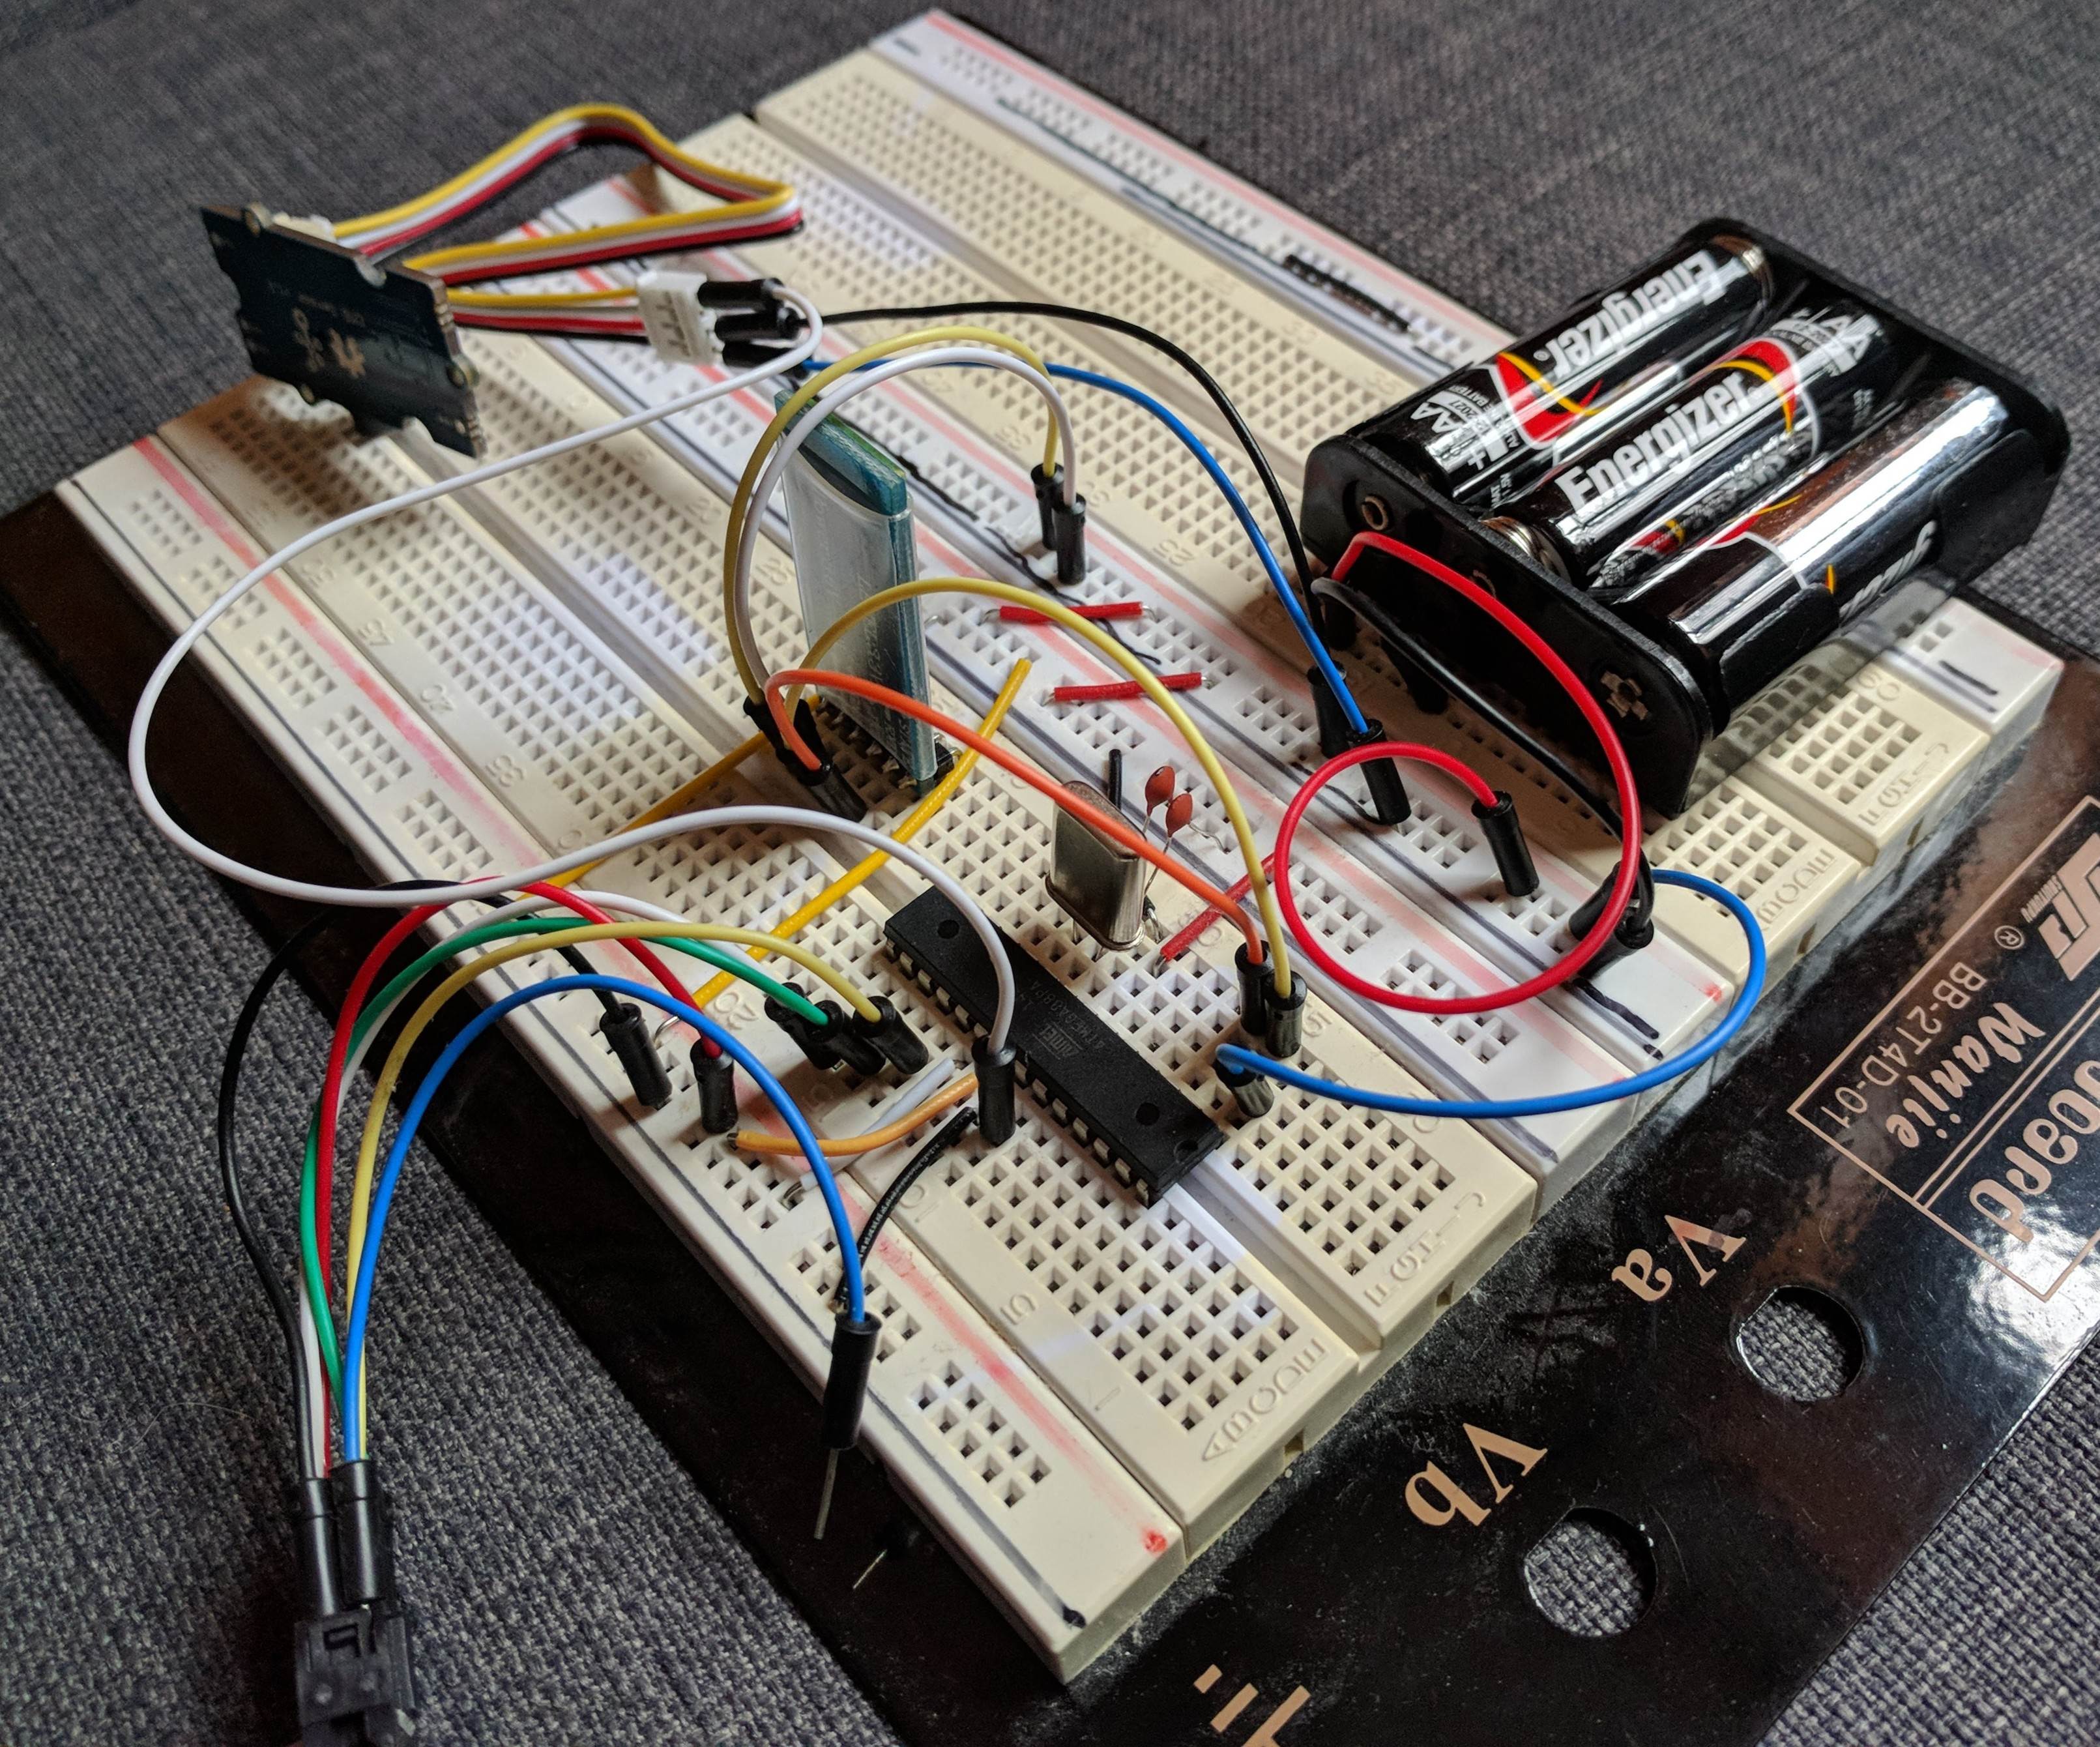
\includegraphics[width=0.7\textwidth]{pics/mikrocontroller.jpg}
	\caption{Foto der aufgebauten Schaltung auf einem Breadboard}
	\label{fig:mikrocon}
\end{figure}
\tocless\subsubsection{Entwicklung des Programms auf dem Mikrocontroller}
\renewcommand{\listingscaption}{Quellcode}
 \begin{longlisting}
 \cfile{../Softwareprodukt/Mikrocontroller/SchlaganfallRehaMotivationsGeraet/SchlaganfallRehaMotivationsGeraet/main.c}
 \caption{Das Programm für den Mikrocontroller}
 \label{listing:mikrocontroller}
 \end{longlisting}
 
\newpage
\setcounter{subsection}{5}
\setcounter{subsubsection}{0}
\tocless\subsubsection{Grundlegender Aufbau und Konzept der App}
\begin{multicols}{2}
\begin{figure}[H]
	\centering
	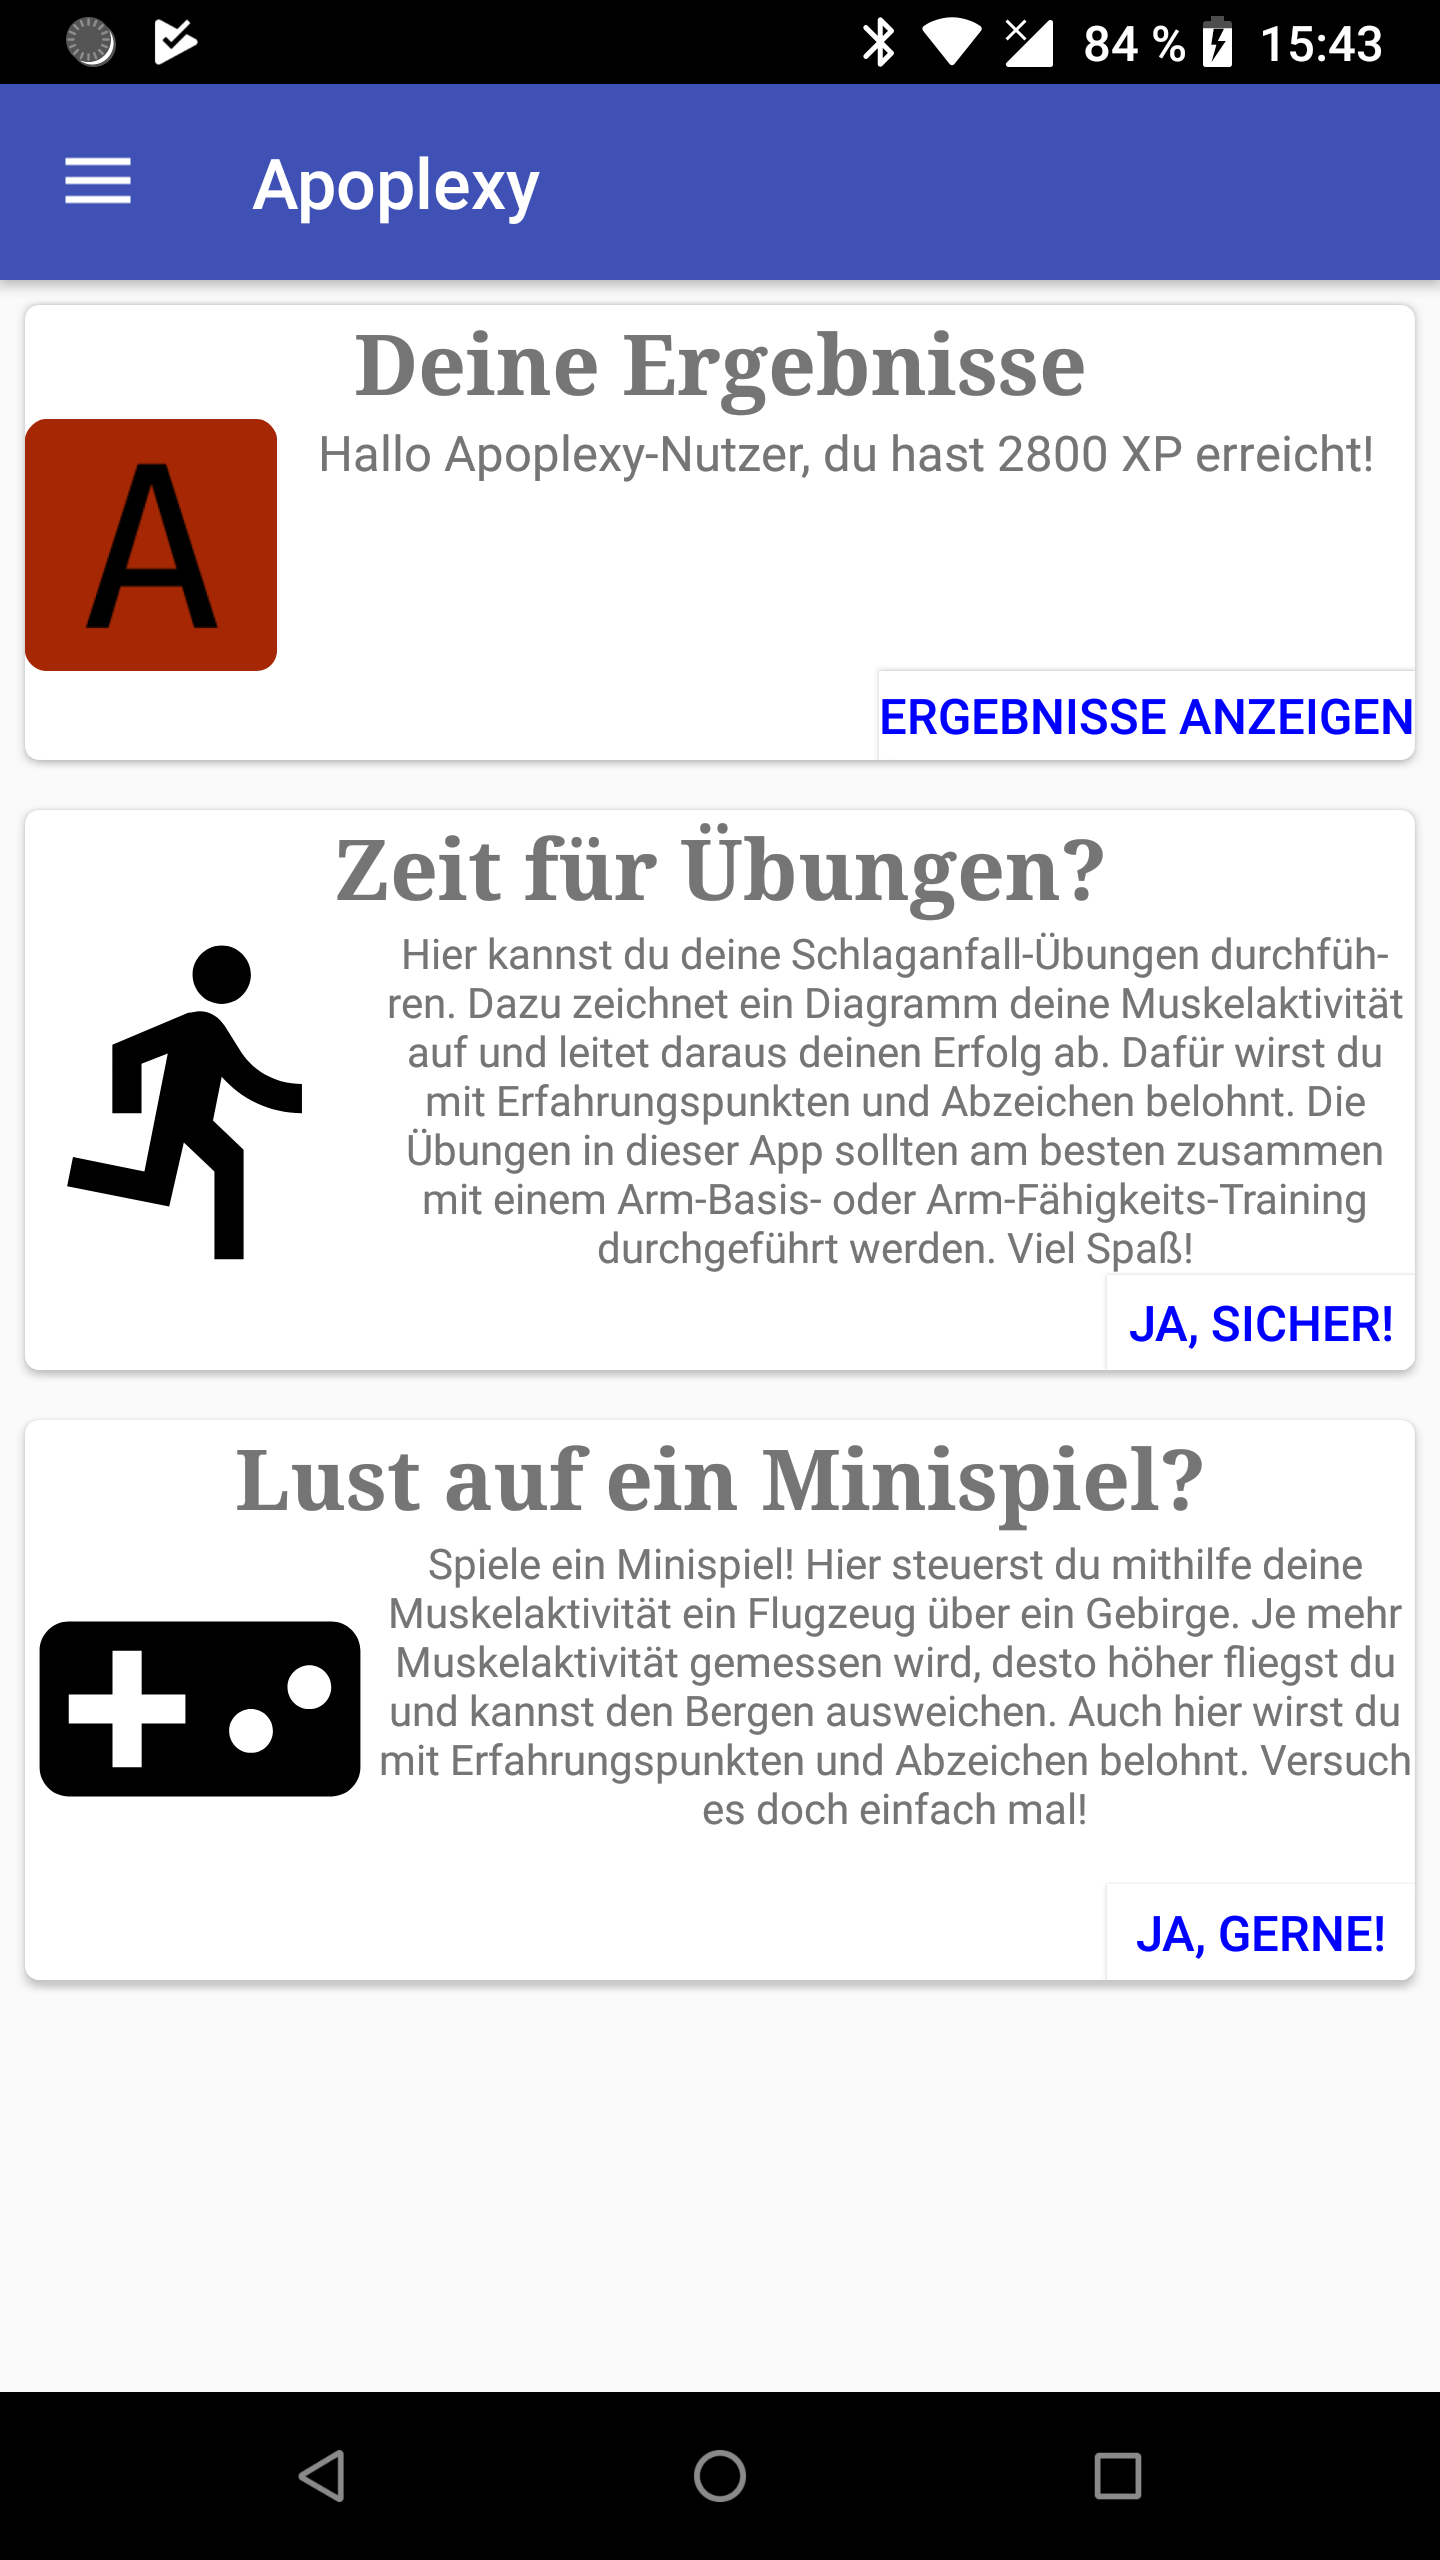
\includegraphics[scale=0.1]{pics/device-home.png}
	\caption{Die Startseite der App}
\end{figure}
\begin{figure}[H]
	\centering
	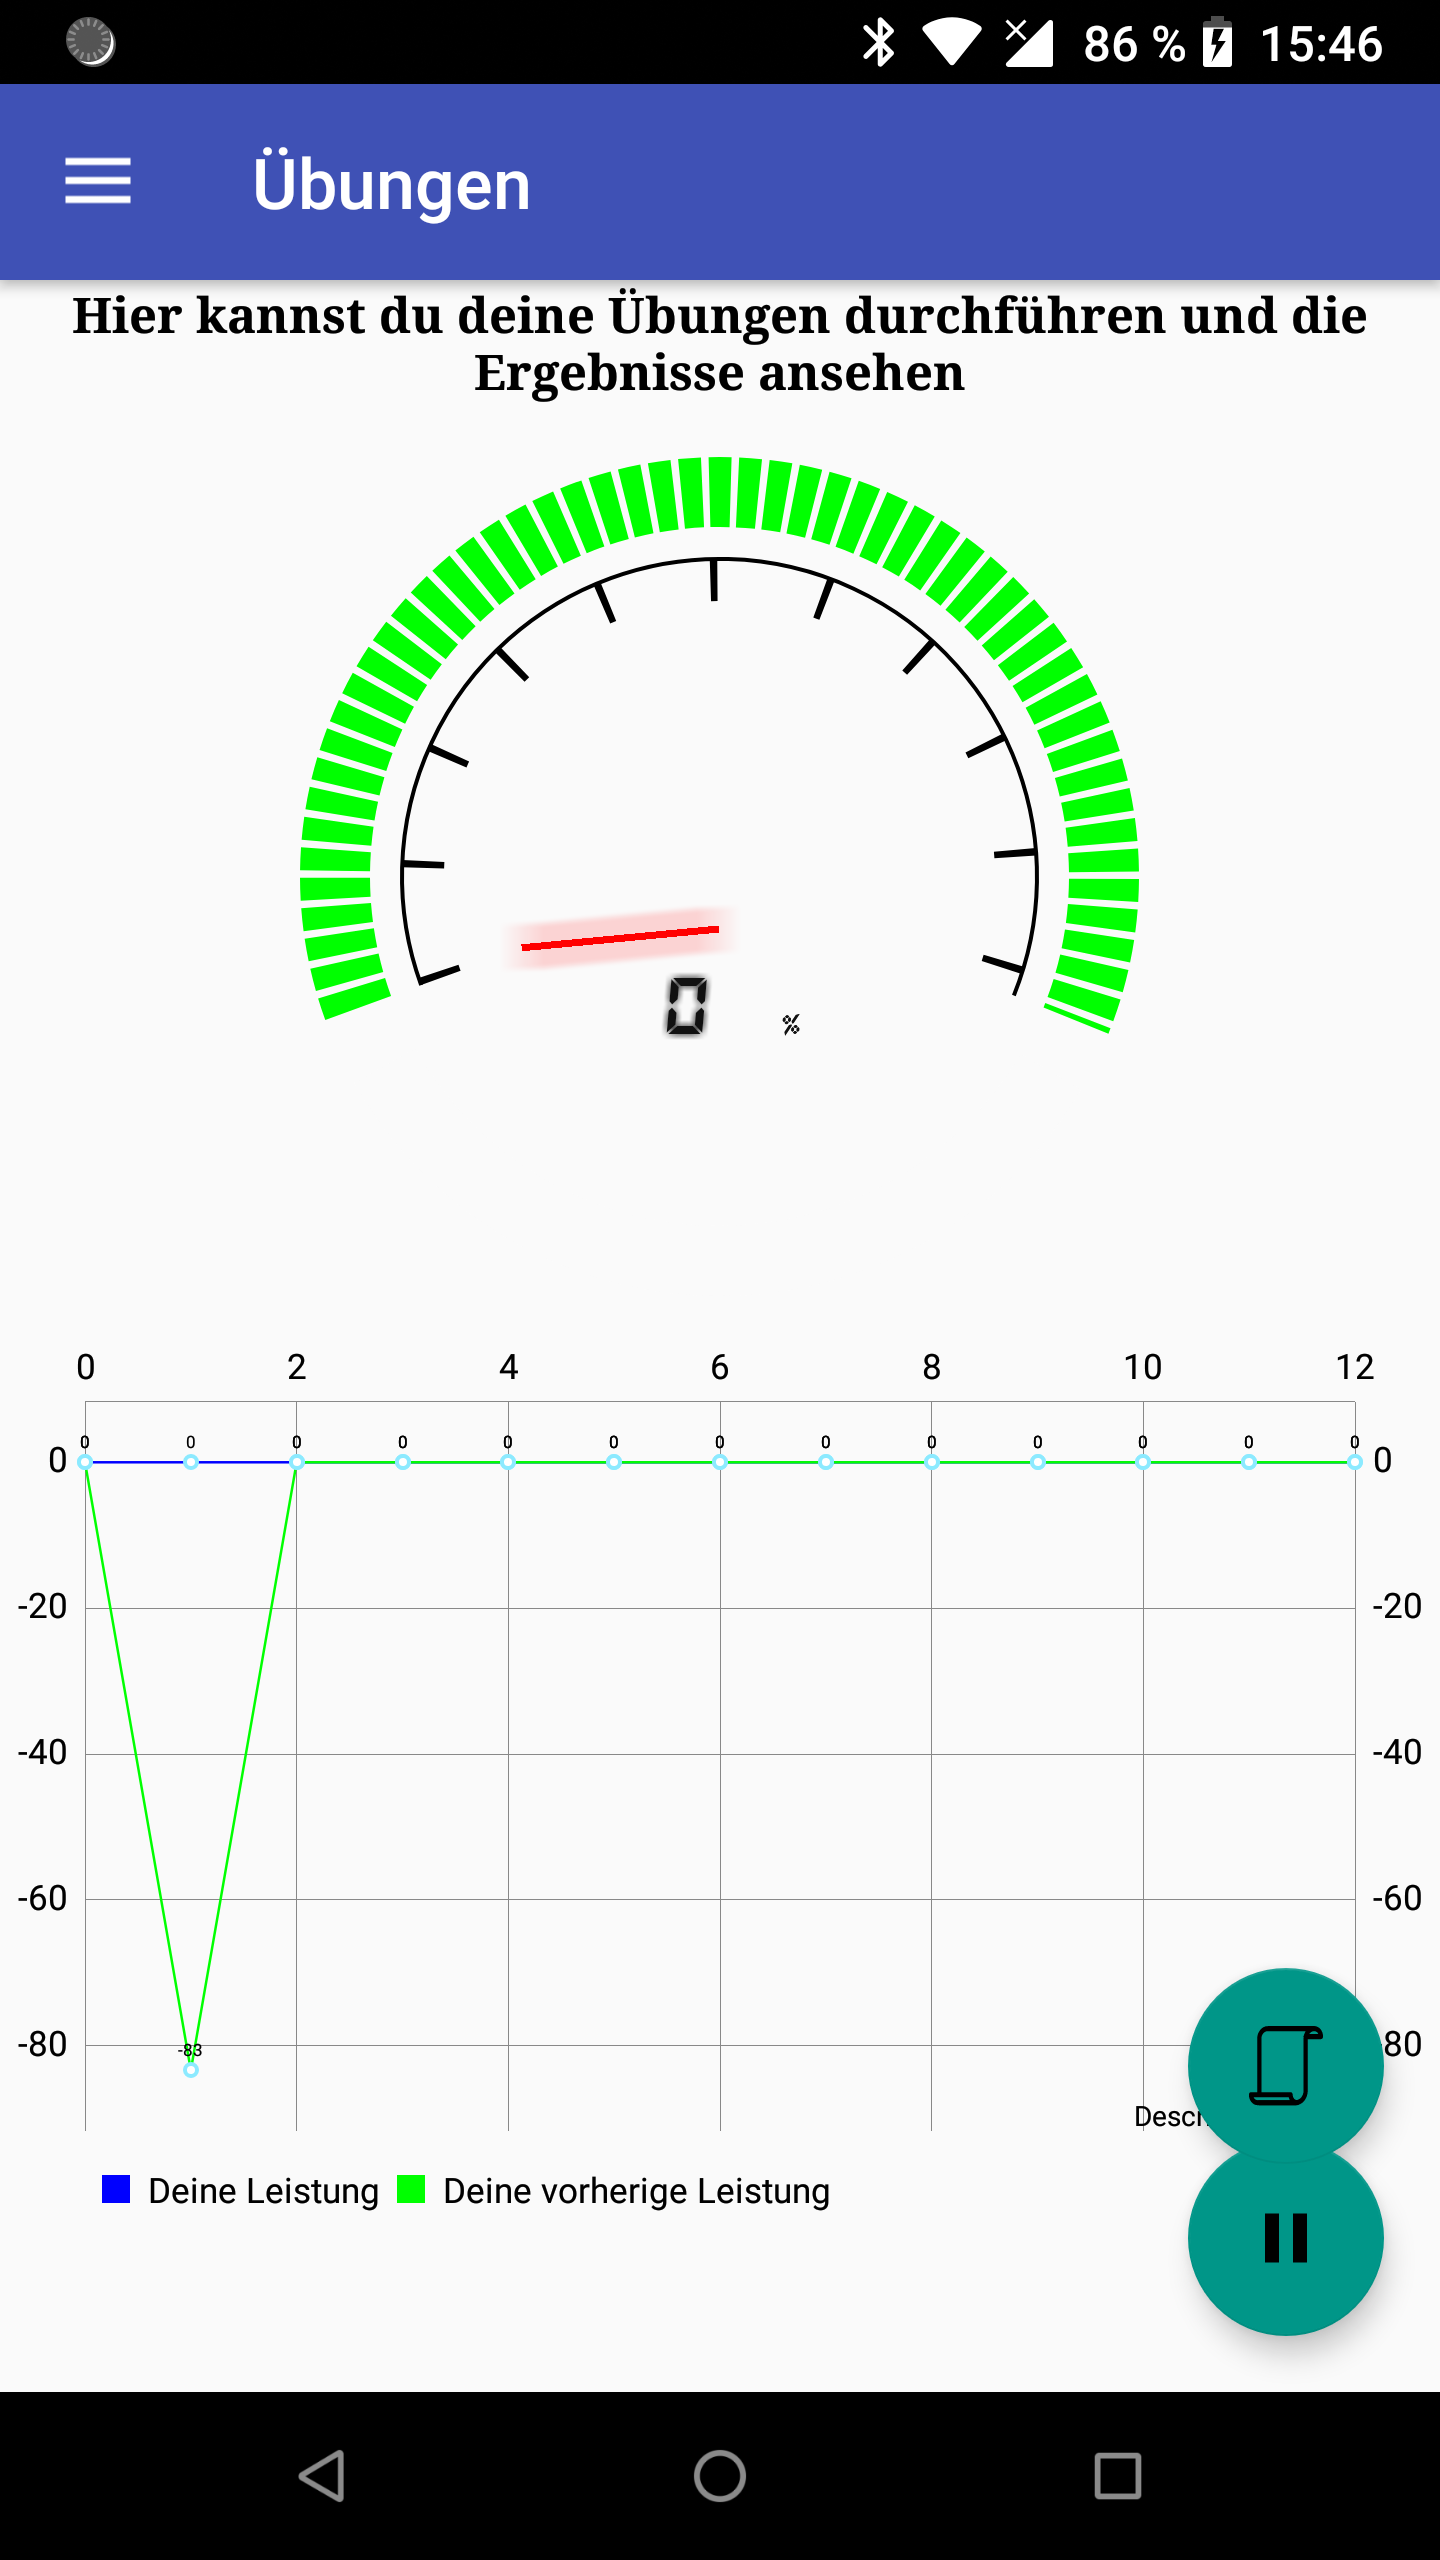
\includegraphics[scale=0.1]{pics/device-exercise.png}
	\caption{Die Übungsseite der App}
\end{figure}
\begin{figure}[H]
	\centering
	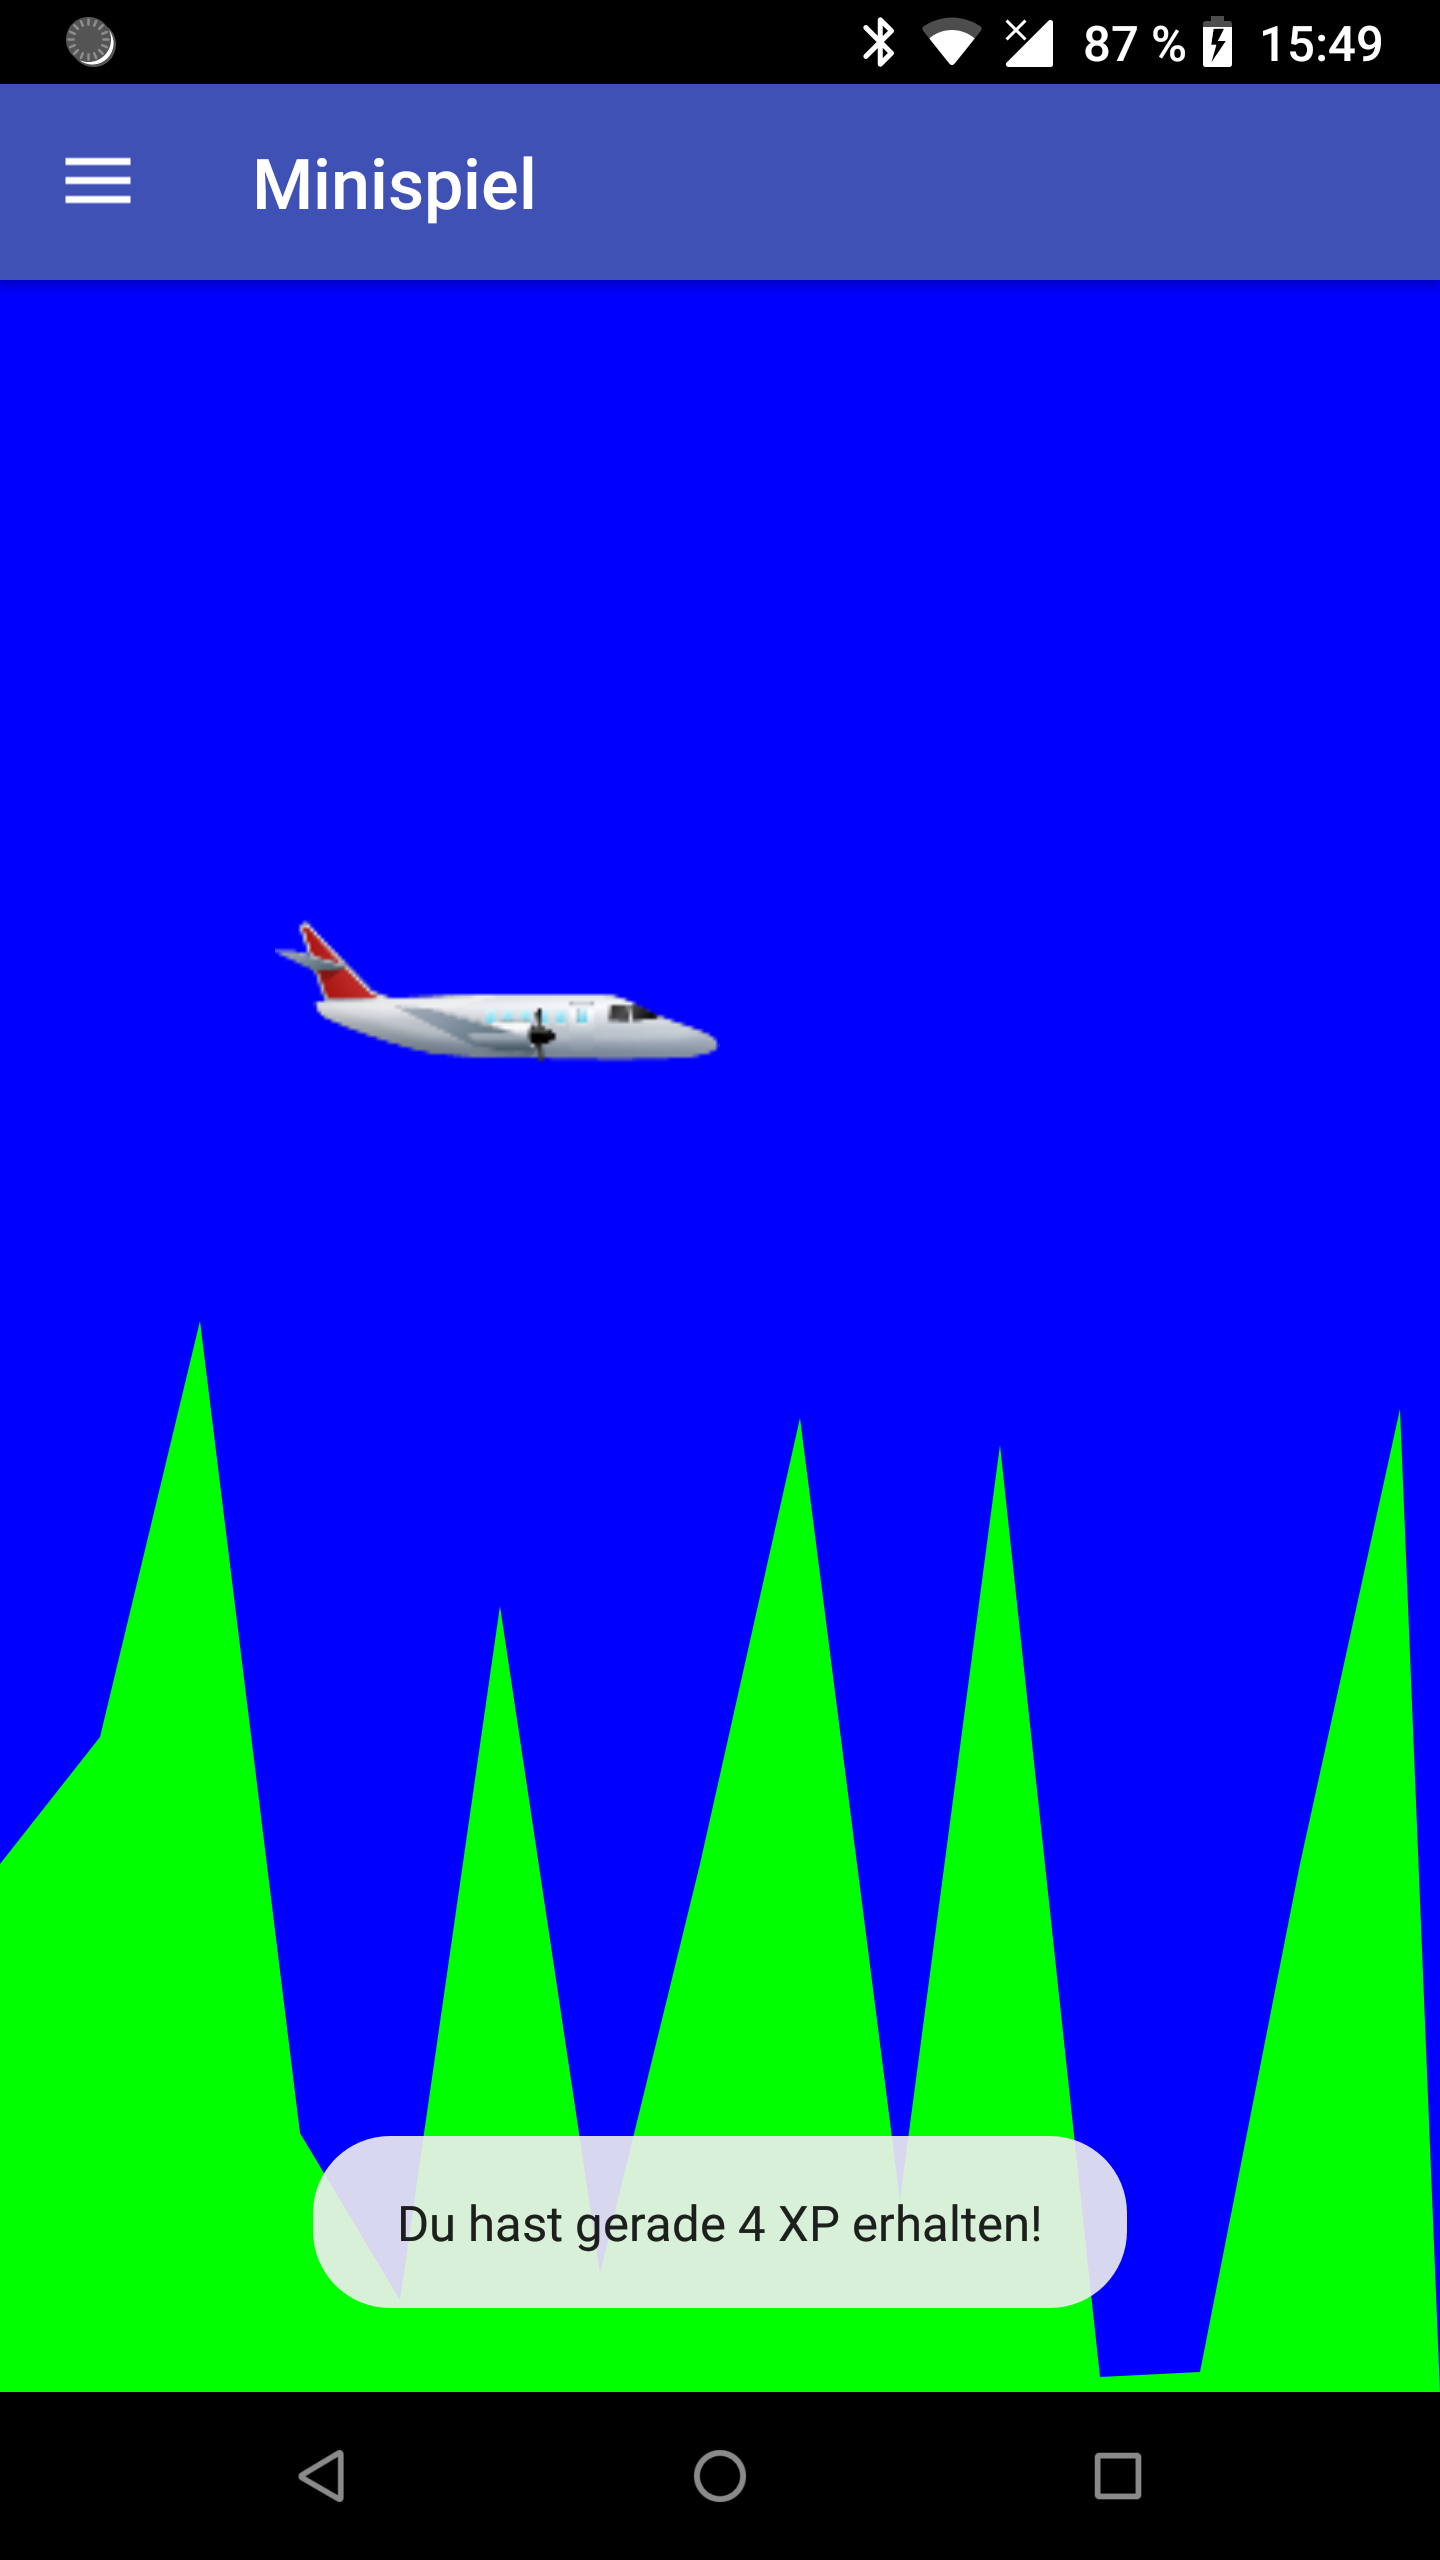
\includegraphics[scale=0.1]{pics/device-game.png}
	\caption{Das Minispiel}
\end{figure}
\begin{figure}[H]
	\centering
	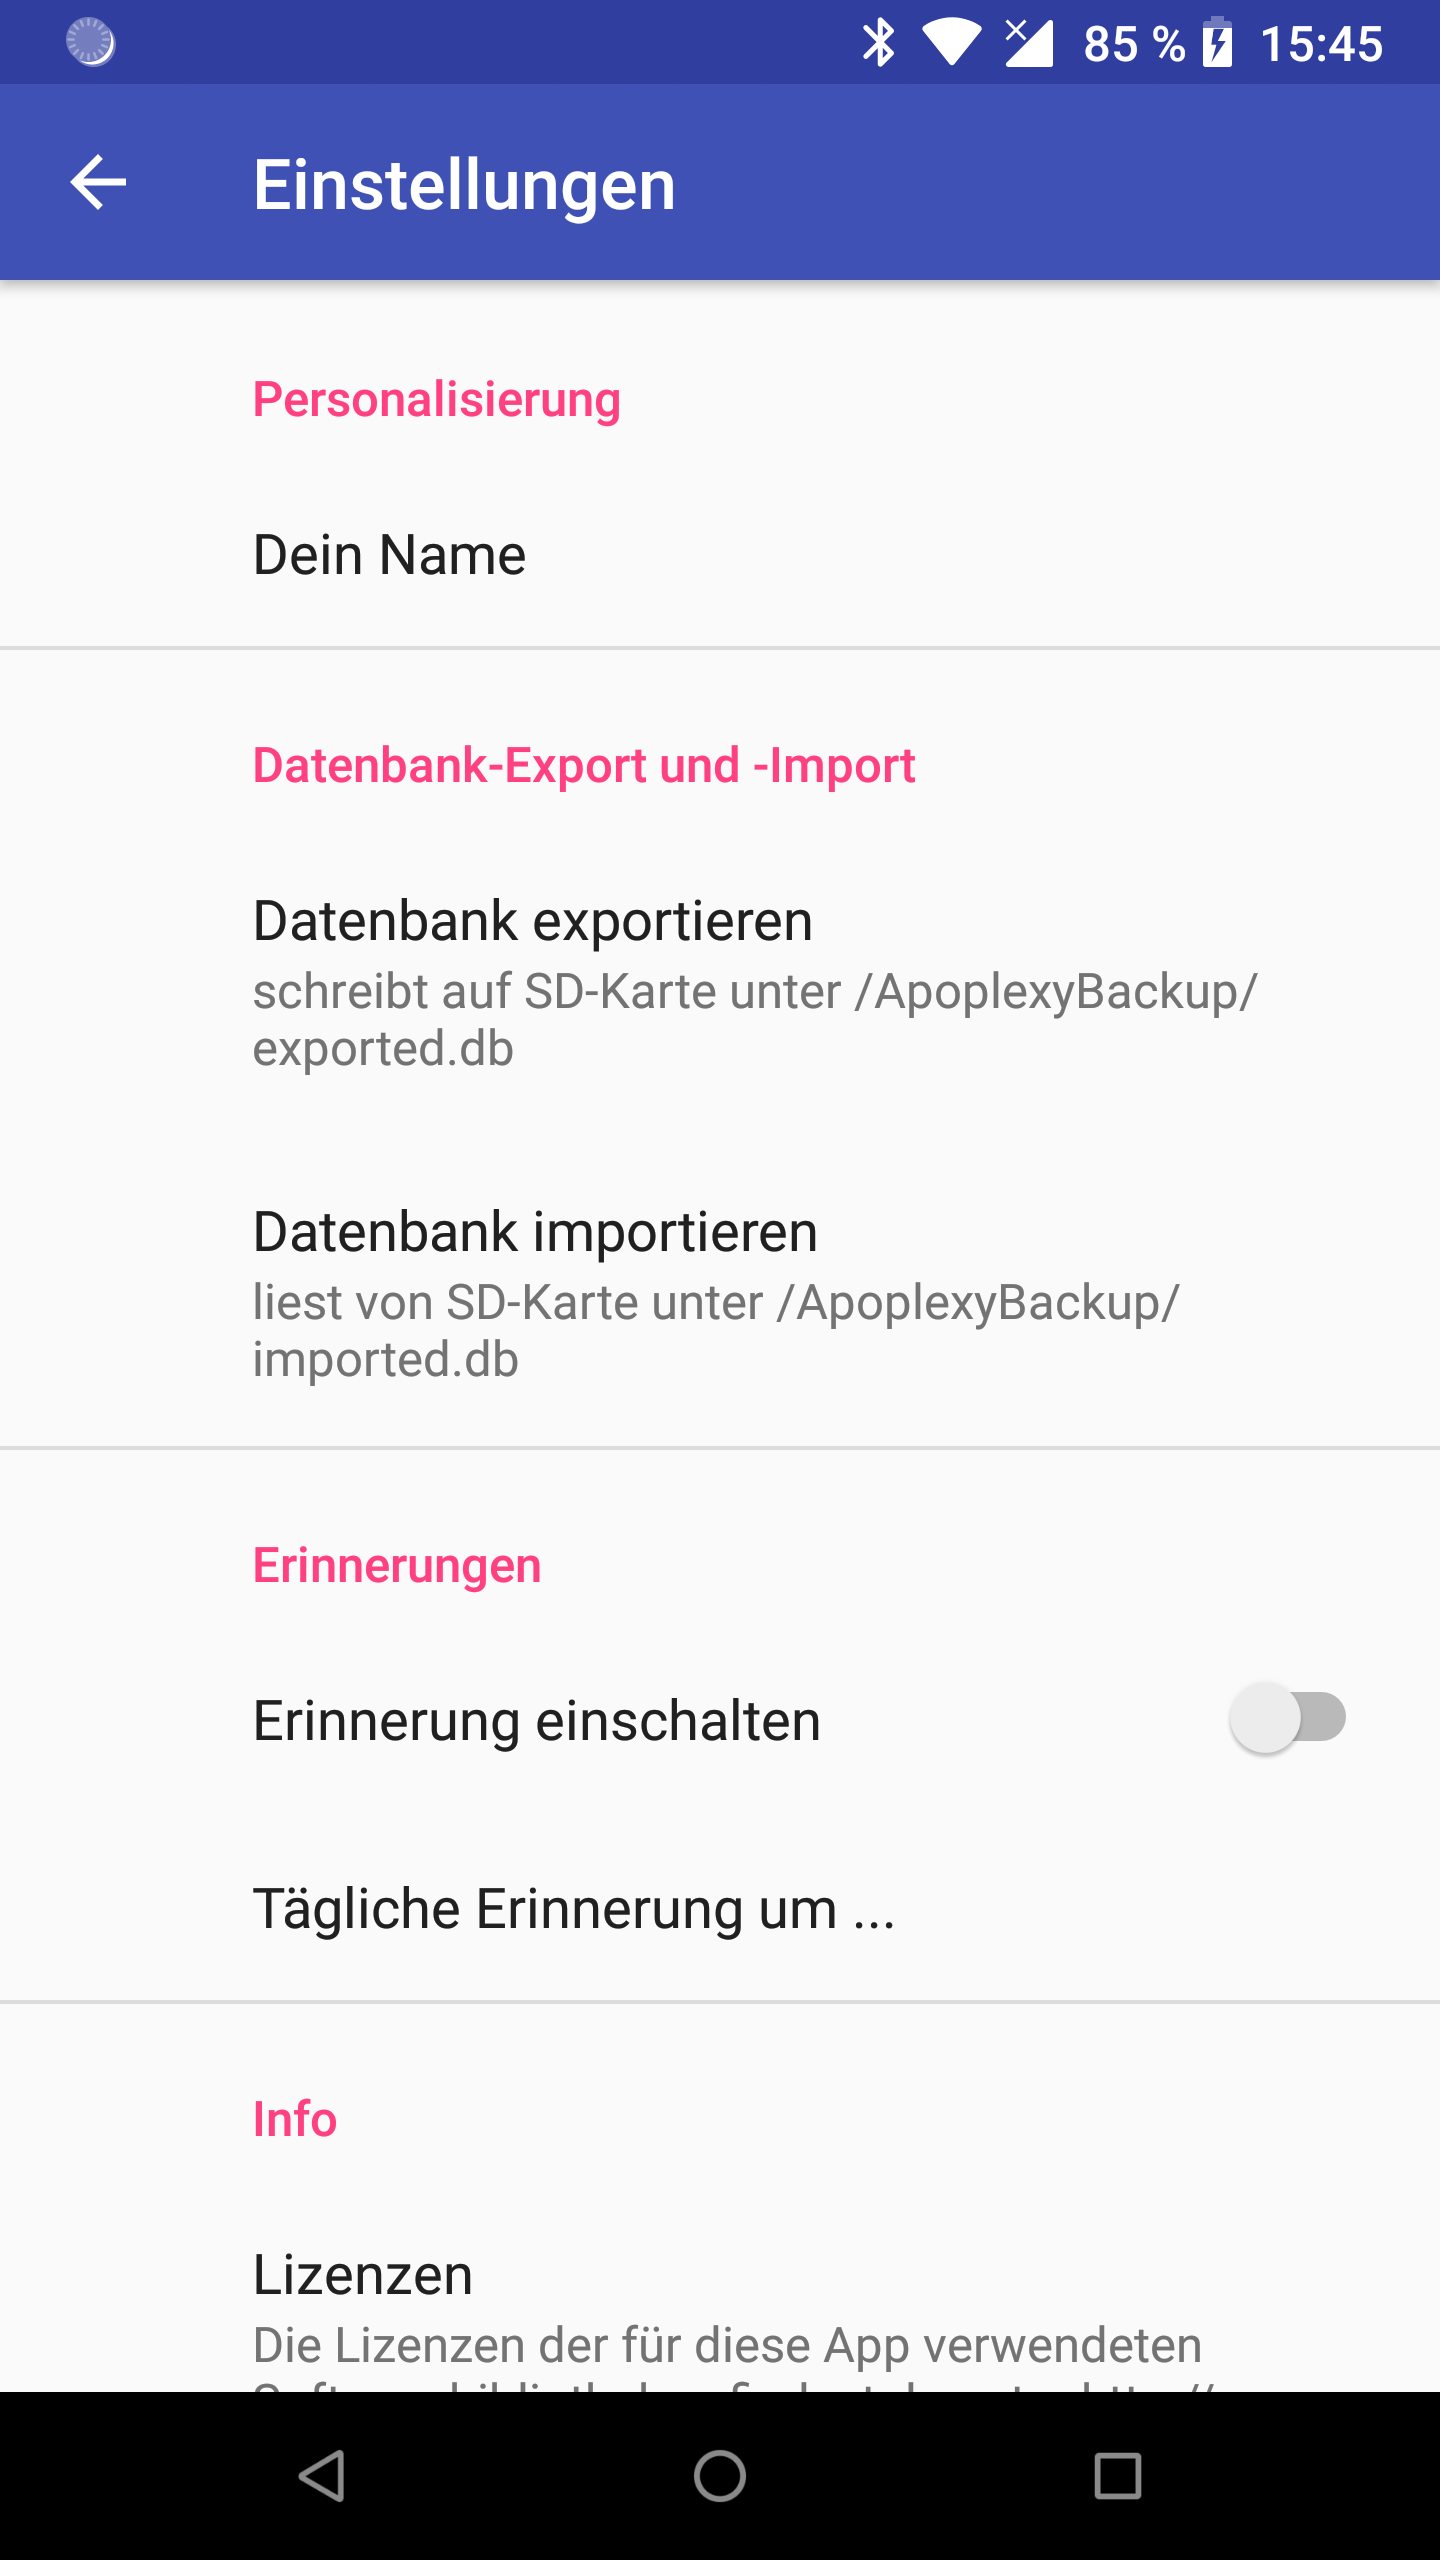
\includegraphics[scale=0.1]{pics/device-settings.png}
	\caption{Die Einstellungsseite der App}
\end{figure}
\begin{figure}[H]
	\centering
	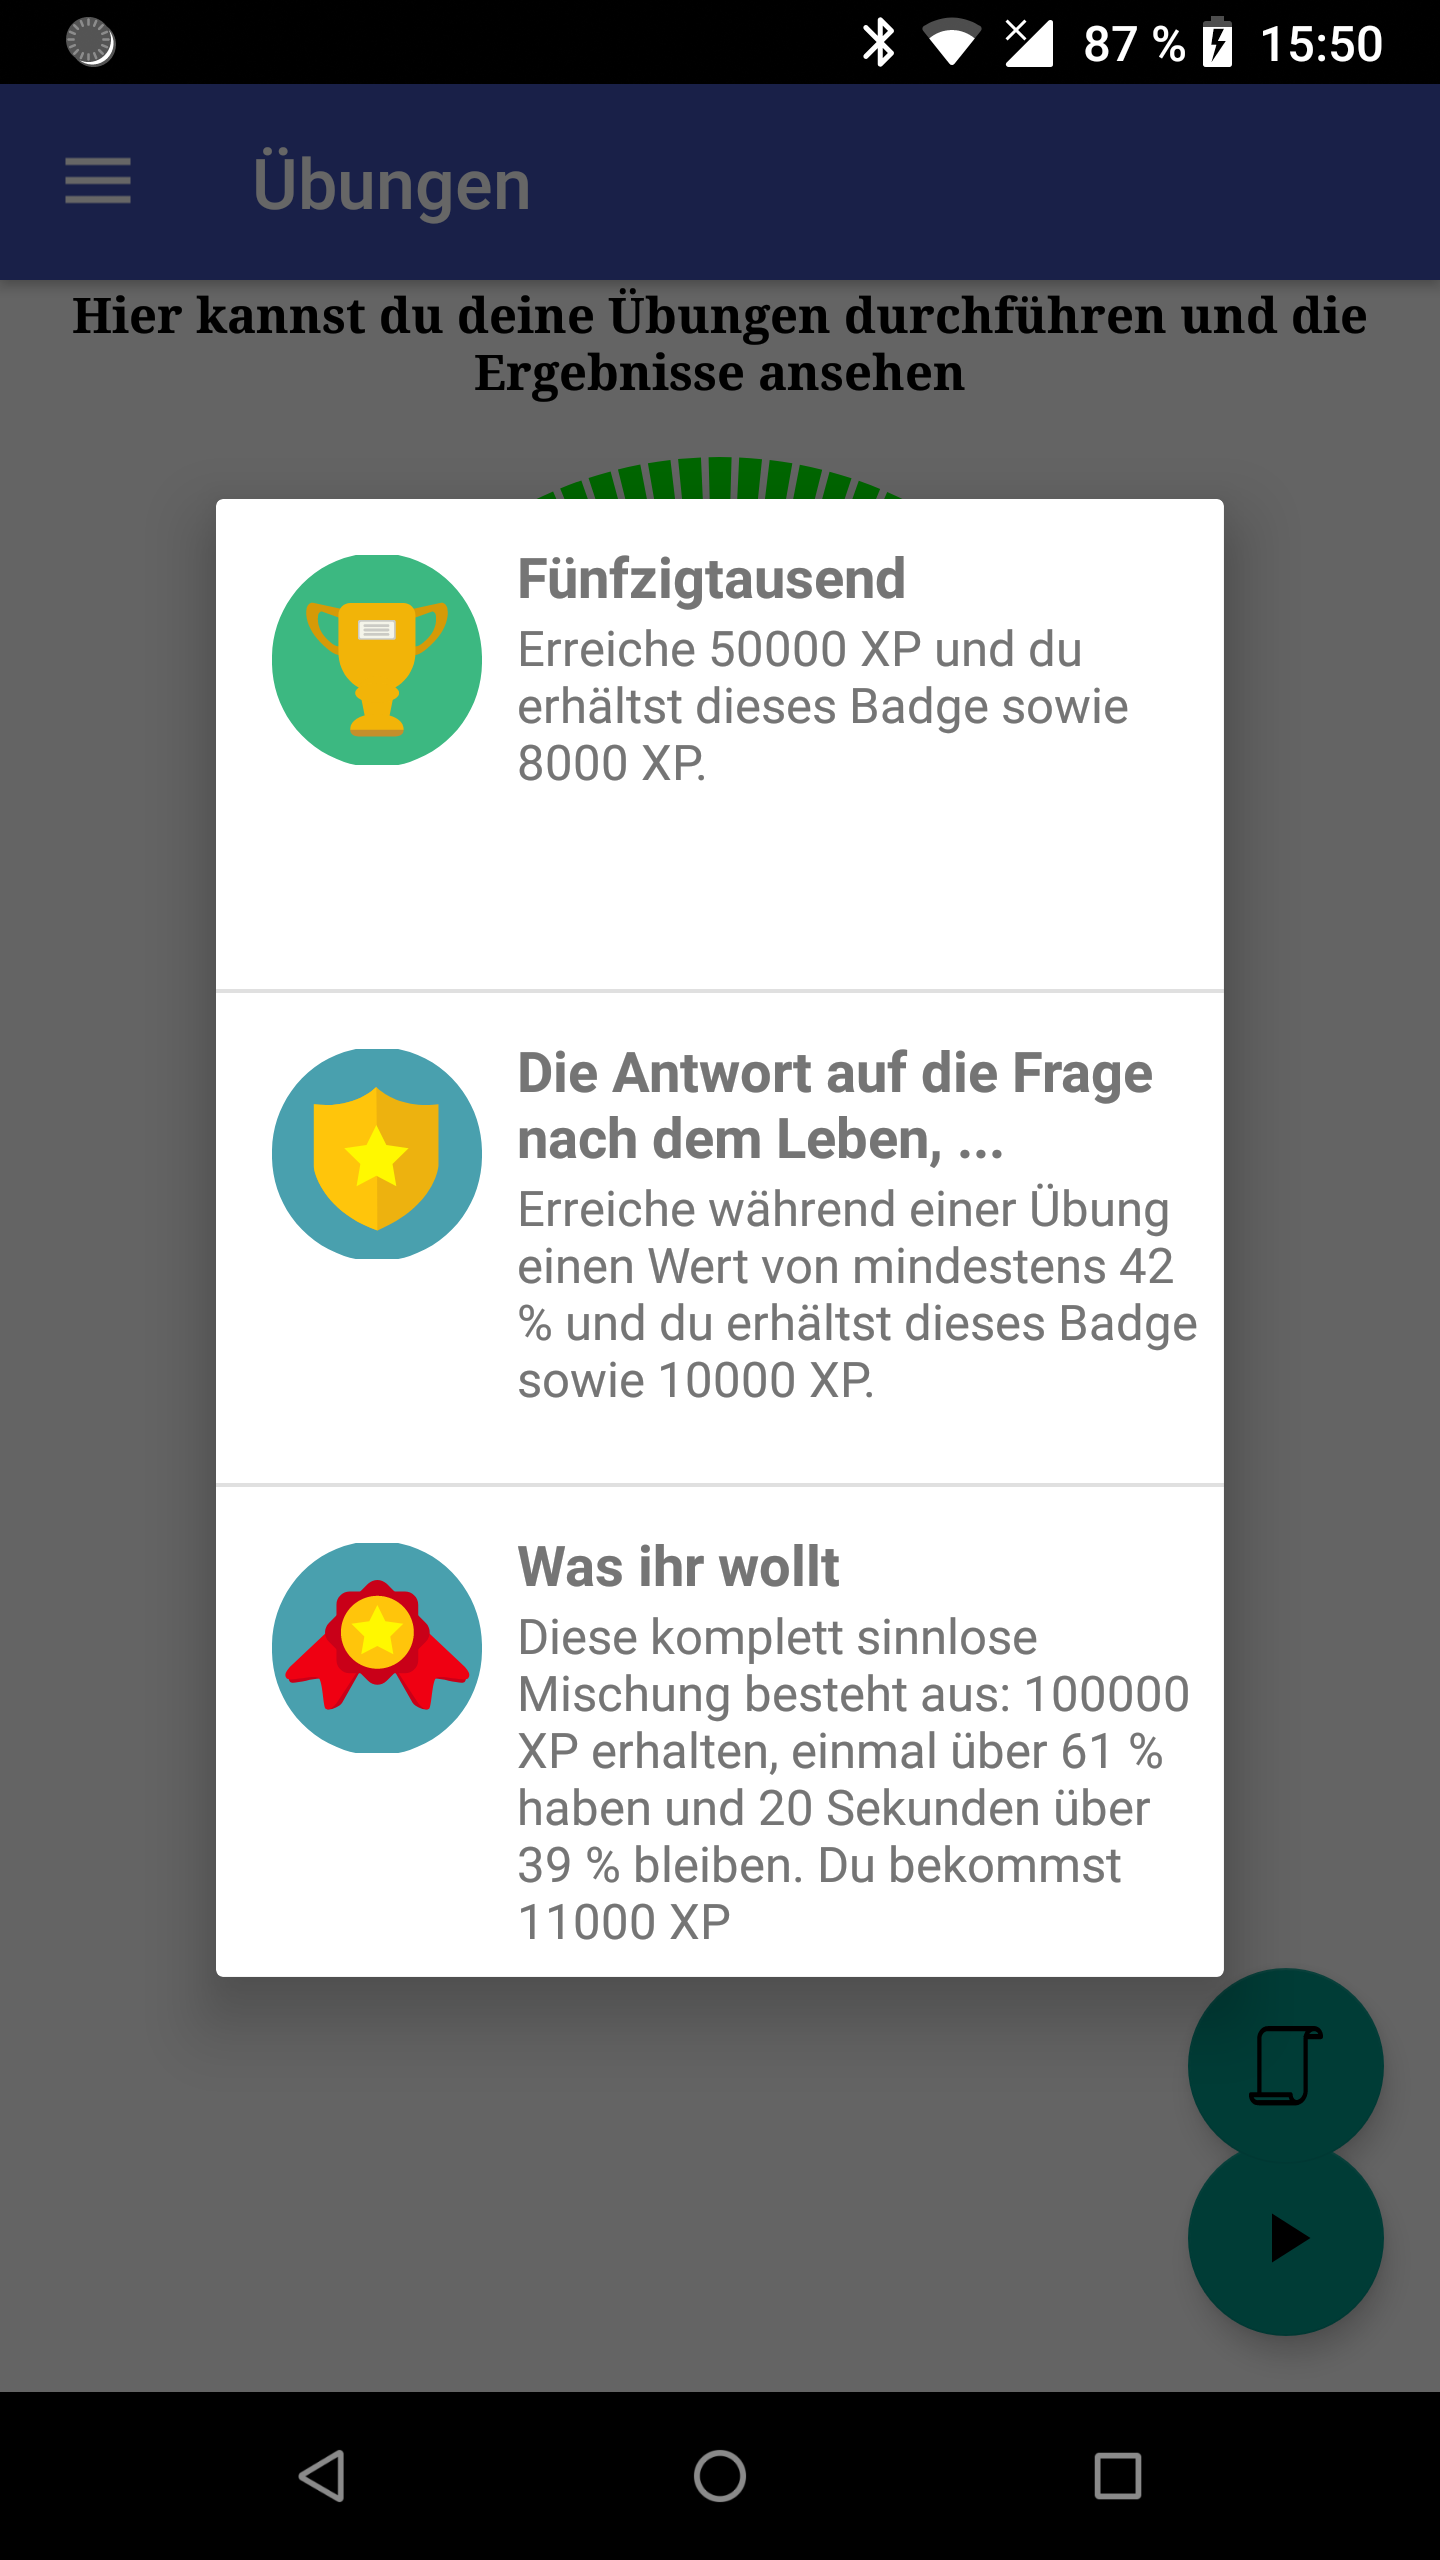
\includegraphics[scale=0.1]{pics/device-badges.png}
	\caption{Die Liste der verfügbaren Quests}
\end{figure}
\begin{figure}[H]
	\centering
	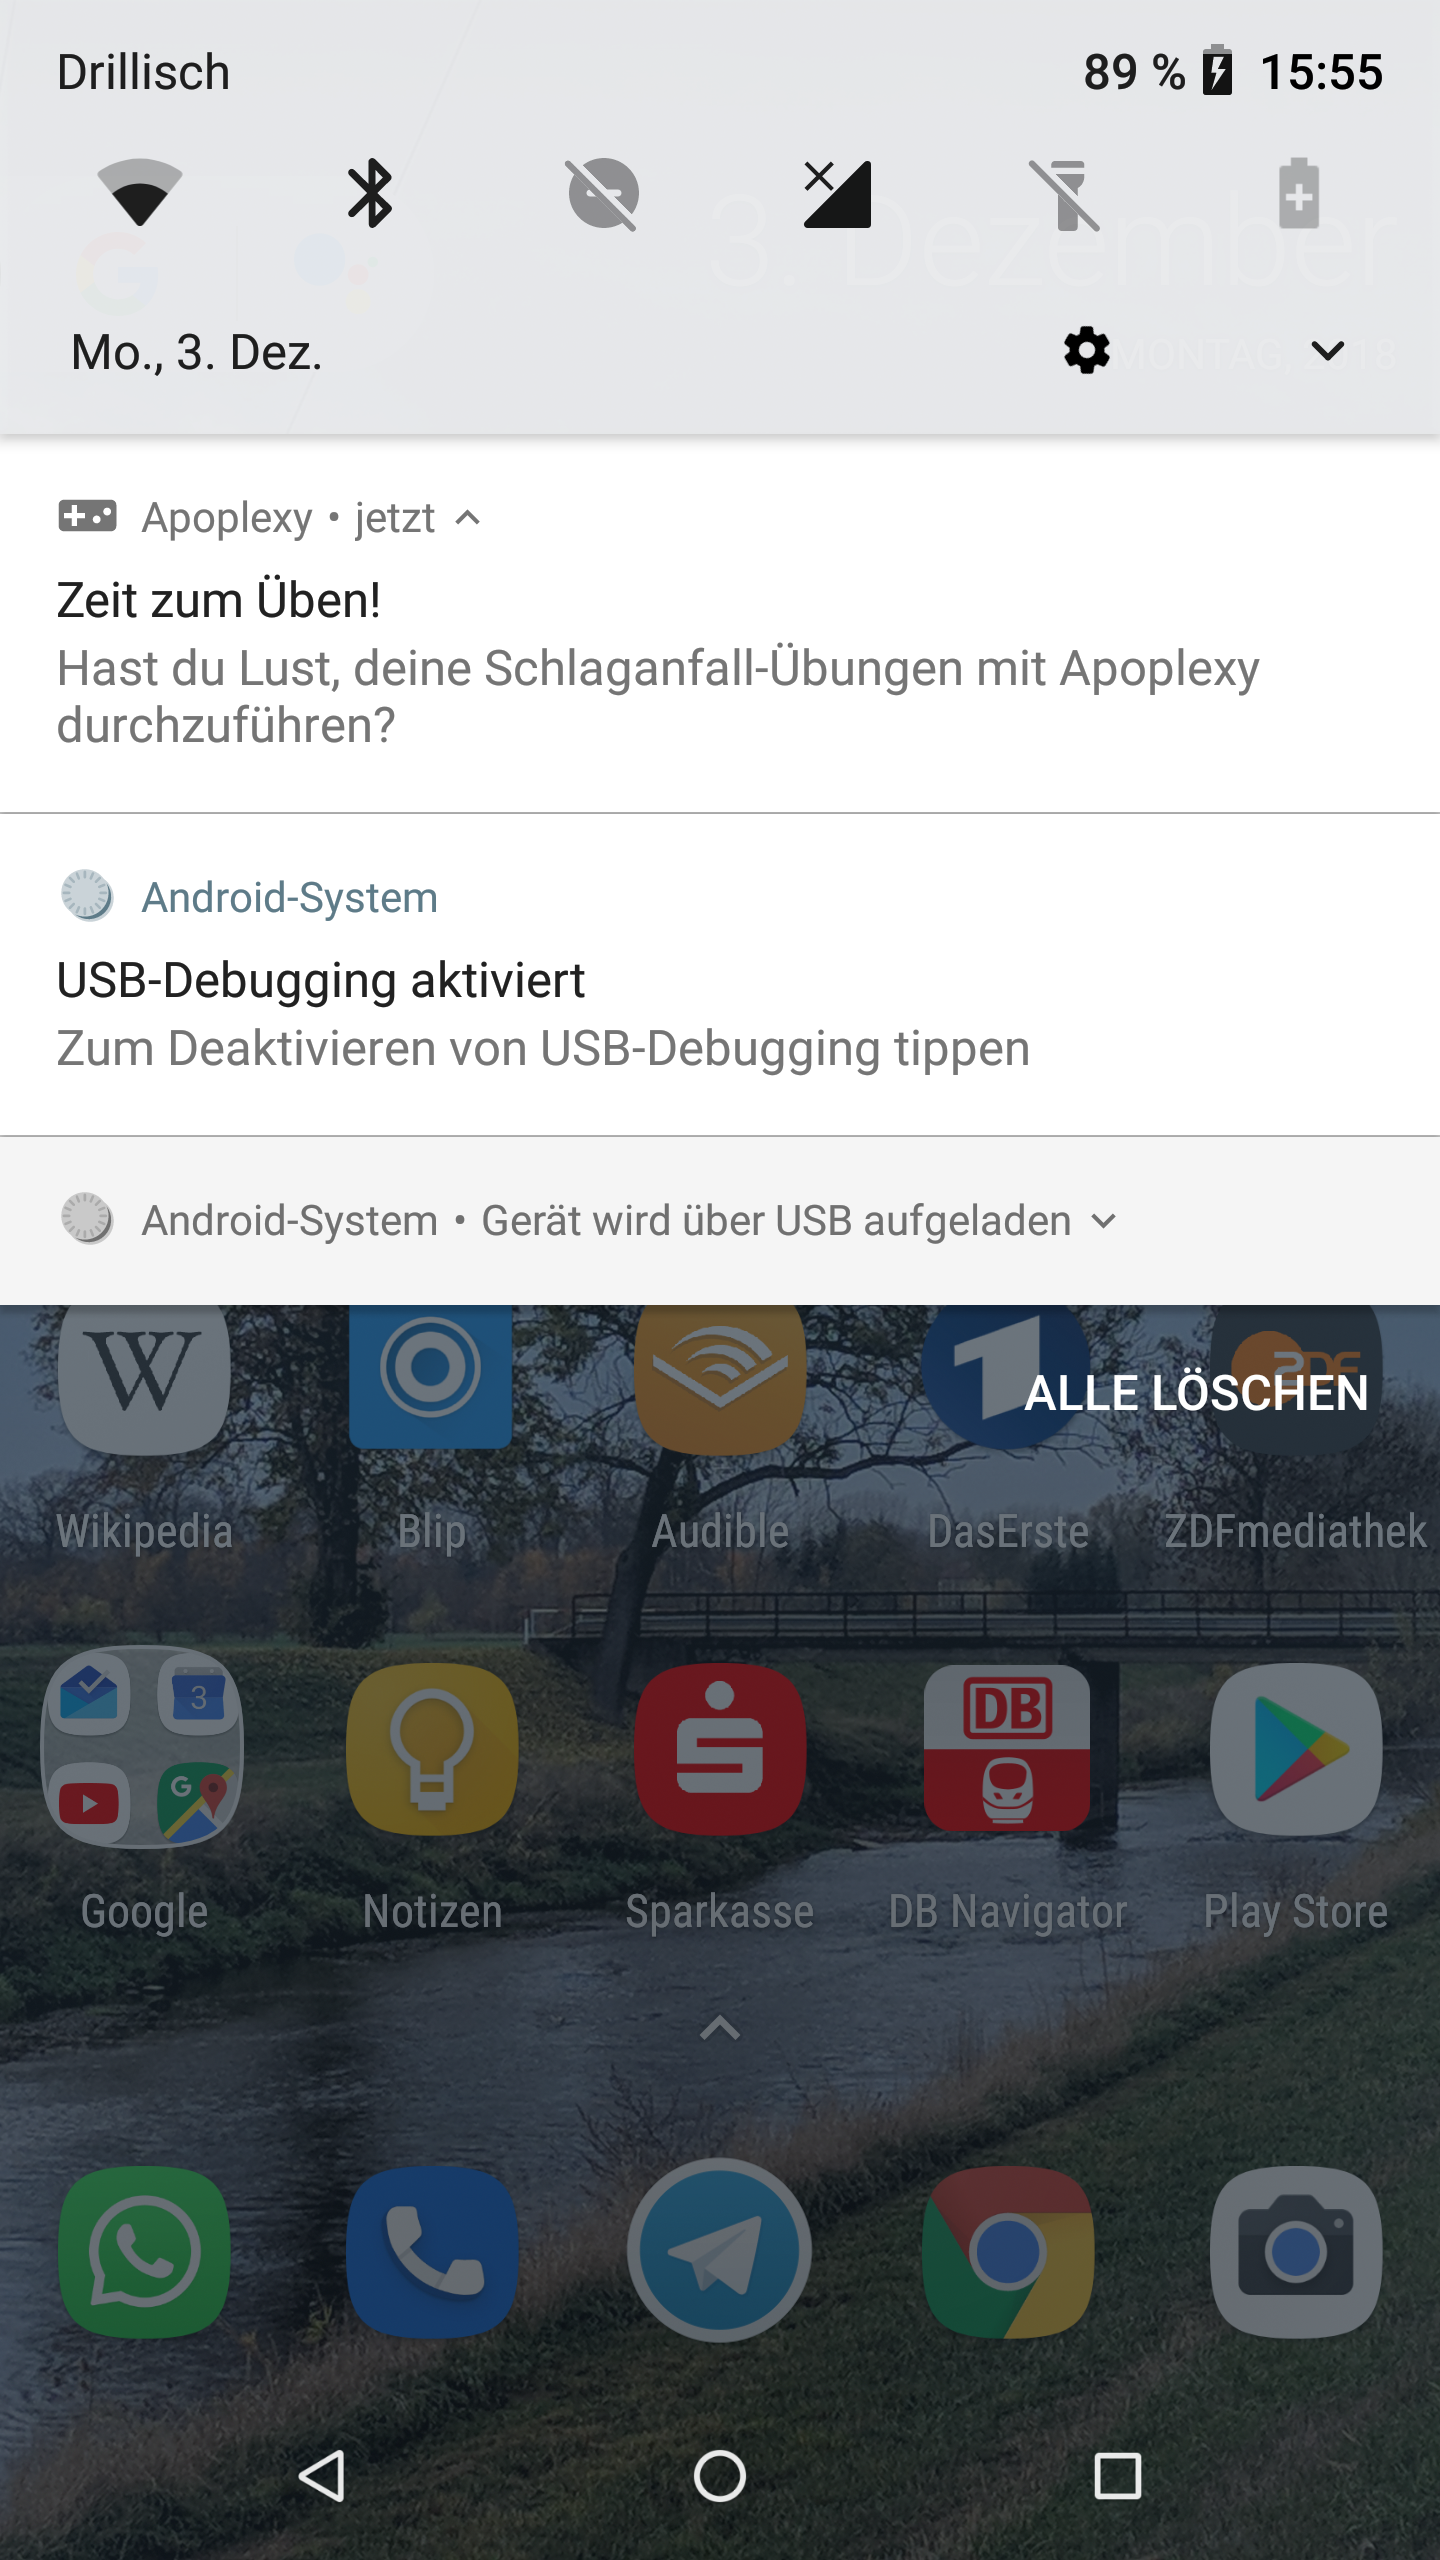
\includegraphics[scale=0.1]{pics/device-notification.png}
	\caption{Eine Übungsbenachrichtigung}
\end{figure}
\end{multicols}

\begin{figure}[H]
	\centering
	\includesvg[width=\textwidth]{pics/apoplexy-uml}
	\caption{UML-Diagramm der App}
\end{figure}

\tocless\subsubsection{Kommunikation mit dem Mikrocontroller}
\begin{longlisting}
	\kotlinfile{../Softwareprodukt/App/app/src/main/java/de/lukasrost/apoplexy/BluetoothNoService.kt}
	\caption{Die \texttt{BluetoothNoService}-Klasse mit der Bluetooth-Funktionalität}
	\label{listing:bluetooth}
\end{longlisting}

\tocless\subsubsection{Konzept und programmiertechnische Umsetzung des Minispiels}
\begin{longlisting}
	\kotlinfile{../Softwareprodukt/App/app/src/main/java/de/lukasrost/apoplexy/game/PlaneGameView.kt}
	\caption{Die \texttt{PlaneGameView}-Klasse mit der Implementierung des Minispiels}
	\label{listing:game}
\end{longlisting}

\tocless\subsubsection{Umsetzung der Gamification in der App}
\begin{longlisting}
	\kotlinfile{../Softwareprodukt/App/app/src/main/java/de/lukasrost/apoplexy/helpers/GamificationGraderHelper.kt}
	\caption{Die \texttt{GamificationGraderHelper}-Klasse mit den Gamification-Bewertungsfunktionen}
	\label{listing:gamification}
\end{longlisting}

\newpage
\section*{Eidesstattliche Erklärung}
Hiermit erkläre ich an Eides Statt, dass ich meine Seminarfacharbeit \glqq Entwicklung eines Gamification - basierten Unterstützungs- und Motivationsgeräts zur Rehabilitation von Schlaganfall-Patienten\grqq ~ selbstständig und nur unter Verwendung der angegebenen Literatur und Hilfsmittel verfasst habe. Außerdem erkläre ich, dass ich alle wörtlich oder sinngemäß aus fremden Werken entnommenen Stellen als solche kenntlich gemacht habe.\\ \\
Die vorliegende Arbeit entspricht in ihrer Vollständigkeit der auf dem gegebenenfalls beigelegten USB-Stick gespeicherten digitalen Version.
\\ \\
Erfurt, 20. Dezember 2018
\\ \\
\begin{center}
\begin{tabular}{@{}l@{}}\hline
$\: \: \:$ Lukas Rost $\: \: \:$
\end{tabular}
\end{center}

\newpage
\section*{Digitale Version}
\vspace{2cm}
\hspace{0.5cm}
\begin{tikzpicture}[x=12.5cm,y=12.5cm]
\draw (0,0) rectangle (1,1);
\end{tikzpicture}

\end{document}
